\documentclass[11pt,a4paper,twoside]{article}

% LaTeX-Umsetzung der "Richtlinien f�r Projekt- und Diplomarbeiten"
% der LFE Medieninformatik, LMU M�nchen. (Autor: Richard Atterer, 27.9.2006, 23.10.2007), Bug-Fixing Mark Kaczkowski (23.6.2008)

\usepackage[T1]{fontenc} % sonst geht \hyphenation nicht mit Umlauten
\usepackage[latin1]{inputenc} % man kann schreiben ����, statt "a"o"u"s
%\usepackage[utf8]{inputenc} % wie oben, aber UTF-8 als Encoding statt ISO-8859-1 (latin1)
\usepackage[english]{babel} % deutsche Trennregeln, "Inhaltsverzeichnis" etc.
%\usepackage{ngerman} % Alternative zum Babel-Paket oben
\usepackage{mathptmx} % Times-Roman-Schrift (auch f�r mathematische Formeln)
\usepackage{enumitem} 
\usepackage{cite}
\usepackage{threeparttable}
\usepackage{caption}
\usepackage{subcaption}

% Zum Setzen von URLs
\usepackage{color}
\definecolor{darkred}{rgb}{.25,0,0}
\definecolor{darkgreen}{rgb}{0,.2,0}
\definecolor{darkmagenta}{rgb}{.2,0,.2}
\definecolor{darkcyan}{rgb}{0,.15,.15}
\usepackage[plainpages=false,bookmarks=true,bookmarksopen=true,colorlinks=true,
  linkcolor=darkred,citecolor=darkgreen,filecolor=darkmagenta,
  menucolor=darkred,urlcolor=darkcyan]{hyperref}

% pdflatex: Bilder in den Formaten .jpeg, .png und .pdf
% latex: Bilder im .eps-Format
\usepackage{graphicx}

\usepackage{fancyhdr} % Positionierung der Seitenzahlen
\fancyhead[LE,RO,LO,RE]{}
\fancyfoot[CE,CO,RE,LO]{}
\fancyfoot[LE,RO]{\Roman{page}}
\renewcommand{\headrulewidth}{0pt}
\setlength{\headheight}{13.6pt} % behebt headheight Warning

% Korrektes Format f�r Nummerierung von Abbildungen (figure) und
% Tabellen (table): <Kapitelnummer>.<Abbildungsnummer>
\makeatletter
\@addtoreset{figure}{section}
\renewcommand{\thefigure}{\thesection.\arabic{figure}}
\@addtoreset{table}{section}
\renewcommand{\thetable}{\thesection.\arabic{table}}
\makeatother

\sloppy % Damit LaTeX nicht so viel �ber "overfull hbox" u.�. meckert

% R�nder
\addtolength{\topmargin}{-16mm}
\setlength{\oddsidemargin}{25mm}
\setlength{\evensidemargin}{35mm}
\addtolength{\oddsidemargin}{-1in}
\addtolength{\evensidemargin}{-1in}
\setlength{\textwidth}{15cm}
\addtolength{\textheight}{34mm}
%________________________________________________________


\begin{document}

\pagestyle{empty} % Vorerst keine Seitenzahlen
\pagenumbering{alph} % Unsichtbare alphabetische Nummerierung

\begin{center}
\textsc{Ludwig-Maximilians-Universit\"at M\"unchen}\\
Department ``Institut f\"ur Informatik''\\
Lehr- und Forschungseinheit Medieninformatik\\
Prof. Dr. Florian Alt

\vspace{5cm}
{\large\textbf{Masterarbeit}}\vspace{.5cm}

\vspace{2cm}
{\huge Design and Development of a Public Display Survey Platform}
\vspace{2cm}

{\large Lukas Ziegler}\\\href{mailto:lukas@lukasziegler.com}{lukas@lukasziegler.com}

\end{center}
\vfill

\begin{tabular}{ll}
Bearbeitungszeitraum: & 6.10.2014 bis 30.04.2015\\
Betreuer: & Prof. Dr. Florian Alt, Jiamin Shi\\
Verantw. Hochschullehrer: & Prof. Dr. Florian Alt
\end{tabular}
%________________________________________________________

\cleardoublepage

    
\section*{Zusammenfassung}

	In den letzten Jahren haben sich Public Displays (PD) in der {\"O}ffentlichkeit stark vermehrt und wurden Teil unseres t{\"a}glichen Lebens. In Einkaufszentren, Bahnh{\"o}fen und Flugh{\"a}fen gibt es immer mehr interaktive Anwendungen f{\"u}r PDs. Ihre Entwicklung erfordert eine umfassende Evaluation, was ein komplexes und zeitintensives Unterfangen ist. Bisher greifen viele der interaktiven Anwendungen noch nicht auf die M{\"o}glichkeit zur{\"u}ck, den R{\"u}ckkanal vom PD zum Display-Anbieter zu nutzen. Um dieses Problem zu l{\"o}sen wurde eine interaktive Umfrage-Plattform entwickelt und eine umfassende Literaturrecherche durchgef{\"u}hrt. \textit{PDSurvey} soll die Durchf{\"u}hrung von Umfragen auf Public Displays erleichtern und als Werkzeug zur weiteren Evaluierung dienen. In dieser Arbeit wird der Entwurf und die Entwicklung unserer Plattform vorgestellt und eine Liste an standardisierten Frageb{\"o}gen vorgeschlagen, welche aus einer umfangreichen Literaturrecherche resultieren. Au{\ss}erdem stellen wir die Ergebnisse unserer Feldstudie vor, in der wir untersucht haben wie Umfragen auf Public Displays wahrgenommen werden und welcher R{\"u}ckkanal am besten f{\"u}r den Nutzer geeignet ist um in digitaler Form auf einen Fragebogen zu antworten.
	Die Ergebnisse lassen folgern, dass eine Mehrheit der Nutzer es vorzieht Umfragen direkt vor Ort zu beantworten. Allerdings hat auch ein Viertel sich gegen die M{\"o}glichkeit entschieden, direkt vor Ort auf den Fragebogen zu antworten. Ein Tablet als R{\"u}ckkanal anzubieten hat sich als beste Option herausgestellt, auch wenn der Benutzer zwischen den Ger{\"a}ten wechseln muss. Umfragen welche direkt auf PDs durchgef{\"u}hrt werden stellen eine sinnvolle Alternative zu Online-Umfragen dar, mit der Einschr{\"a}nkung der sozialen Erw{\"u}nschtheit und der Abnahme der Privatsph{\"a}re.


\selectlanguage{english}
\section*{Abstract}

	In recent years, public displays (PD) have proliferated in public space and become part of our daily lives. New interactive applications for PDs are flourishing in shopping malls, train stations, and airports. Their development requires extensive evaluation, which is a complex and time intensive endeavor. So far, many interactive PDs still lack a feedback channel from display to display provider. To solve this problem an interactive survey platform was developed and an extensive literature review carried out.
	\textit{PDSurvey} aims to facilitate the execution of surveys on public displays and is a toolset for further PD evaluation. In this thesis, the design and development process of our platform is presented and a list of standardized questionnaires proposed, resulting from an extensive literature review. Furthermore, we present the findings of our field study, in which we assessed the general acceptance of questionnaires being conducted in public space and which feedback channels are best suited for users to respond to questionnaires in a digital form.
	The findings imply that a majority of users prefer to complete a survey directly on-site. However, a quarter refrained from using PDs for responding to the questionnaire. Offering the tablet as a feedback channel represented the best choice, even though users have to switch devices. Surveys conducted on public displays are a reasonable alternative to online surveys, with the limitation of social desirability and a decrease in privacy.
	


	% BENEFITS: simplifying evaluation, better scalability, offering a feedback channel, comparison of PDs based on their context

	% potential LIMITATIONS: social desirability, less in-depth responses, decrease of privacy


	% Inspiration for good Abstracts: MyPosition \cite{valkanova2014myposition}, Mueller 2010: Requirements and Design Space for Interactive Public Displays \cite{muller2010requirements}, 


\cleardoublepage

    
\section*{Acknowledgments}

I would like to thank Jiamin Shi, Axel H{\"o}sl, Dr. Julie Wagner, and the entire Mediainformatics chair, for their great spirit and support. It was great to be able to complete my Master studies and thesis at the chair.Additionally, I would like to thank Prof. Dr. Florian Alt, for his guidance, feedback, and the time devoted to my Master's thesis. But abve all, I would like to thank my parents for their continuous support throughout my entire education. Much would not have been possible without their love and care. 



\cleardoublepage

    \section*{Aufgabenstellung} % section* = kein Eintrag ins Inhaltsverzeichnis

\textbf{Development of a Public Display Survey Platform}

\begin{description}
    \item[Problem Statement] Public displays are quickly proliferating in public space. At the same time, interactive applications are still scarce, since their development is costly and the effect on the user - and thus their benefit - is often not clear. Hence, interactive displays applications are usually developed, deployed, and carefully evaluated in research contexts. In most cases, evaluation focusses on particular aspects only, such as user performance, user experience, or social implications, due to the significant effort associated with planning, preparing and conducting public display evaluations.
    \item[Scope of the Thesis] To tackle the aforementioned challenge, the objective of this thesis is to develop a survey tool that allows interactive public display installations to be comprehensively assessed. In a first step, an extensive literature review will be conducted with the aim to identify important aspects of public display deployments - both from a researcher as well as from a practitioners' perspective - as well as to develop an understanding of how these aspects could be addressed through surveys. Based on the literature review, a web-based survey platform will be implemented that can easily be used to evaluate and compare public displays through different channels. Such channels include both evaluation directly at the display or through a (mobile) website that allows participation also via a smartphone or tablet. The platform should allow public display owners to configure their own surveys based on their needs. Optionally, the survey tool itself will be evaluated with an interactive public display application.

    \item[Tasks] 
    (1) conduct a literature review to identify (research) questions that are of interest to researchers and practitioners \newline
(2) produce a comprehensive set of questions that can be used to assess these questions by means of a survey \newline
(3) develop a web-based public display survey platform consisting of (a) an administration interface that allows (groups of) questions to be selected for use within the tool and
(b) a responsive UI that can be rendered on different devices (public display, smartphone, tablet, laptop)

    \item[Requirements] Strong skills in web programming, independent scientific work and creative problem solving, experience in creating questionnaires is a plus.

    \item[Keywords] Public displays, interaction, applications, survey, questionnaires, web

\end{description}

    \vfill % align text to the bottom of the page

    \noindent Ich erkl\"are hiermit, dass ich die vorliegende Arbeit
    selbstst\"andig angefertigt, alle Zitate als solche kenntlich gemacht
    sowie alle benutzten Quellen und Hilfsmittel angegeben habe.

    \bigskip\noindent M\"unchen, \today

    \vspace{4ex}\noindent\makebox[7cm]{\dotfill}


\cleardoublepage

    \pagestyle{fancy}
    \pagenumbering{roman} % Roemische Seitenzahlen
    \setcounter{page}{1}

% Inhaltsverzeichnis erzeugen
\tableofcontents

%Abbildungsverzeichnis erzeugen - normalerweise nicht nötig
%\cleardoublepage
%\listoffigures
%________________________________________________________

\cleardoublepage

% Arabische Seitenzahlen
\pagenumbering{arabic}
\setcounter{page}{1}
% neues Seitenformat
\fancyhead[LE,RO]{\rightmark}
\fancyhead[LO,RE]{\leftmark}
\fancyfoot[LE,RO]{\thepage}


%________________________________________________________

%%%  INTRODUCTION  %%%

    \section{Introduction}
\label{sec:introduction}



\begin{enumerate}
\item nice introduction in paper: valkanova2014myposition
\end{enumerate}



\subsection{Motivation}

Scope for the practical part of the thesis. What is the system supposed to look like. What is the current state of the practical work in research and in the industry. Which partners do we have, where do we want to deploy this system. What are the goals for this evaluation plattform?


  \begin{enumerate}
  \item What are public displays?
  \item 
  \end{enumerate}


\subsection{Research Question}



\subsection{Approach}



\subsection{Overview}







% EXAMPLE TEXT

% \begin{enumerate}[itemsep=0pt] 
% \item option 1
% \item option 2
% \end{enumerate}


%\begin{figure}%[btph]
  %% Datei ``beispielbild.eps'' oder ``beispielbild.png'', zentriert
  %\begin{center}\includegraphics{beispielbild}\end{center}

  %% Datei auf 8cm Breite verkleinert/vergr��ert
  %\includegraphics[width=8cm]{beispielbild}
  %% Datei auf ganze Breite des Texts vergr��ert
  %\includegraphics[width=\columnwidth]{beispielbild}
  %% Datei auf 60% der Textbreite verkleinert/vergr��ert
  %\includegraphics[width=.6\columnwidth]{beispielbild}
  %% Weitere Optionen (Ausschnitt, drehen etc.) in der Doku zum graphicx-Paket

%  \begin{center}\LARGE [BILD]\end{center}
%  \caption{Bildunterschrift}
%  \label{fig:beispielbild}
%\end{figure}

    %Siehe Abbildung \ref{fig:beispielbild} oder einschl\"agige Literatur, z.B.
    %\cite[Seite 6]{Ivory01} oder \cite{NielsenAlertbox}.


% \begin{figure}
%   \begin{center}\LARGE [BILD]\end{center}
%   \caption{Bild}
%   \label{fig:beispielbild3}
% \end{figure}


    

%________________________________________________________

\cleardoublepage % Neue rechte Seite anfangen (nur vor \section)

    \section{Related Work}
\label{sec:related-work}


	The goal of the literature review was to find out how other researchers evaluate public displays. The aim was to identify important aspects of public display deployments - both from a researcher's as well form a practitioner's perspective. Furthermore it was of interest to develop an understanding of how these aspects could be addressed through surveys. 



%%%  REMINDERS  %%%


	% The introduction should be focused on the thesis question(s).  All cited work should be directly relevent to the goals of the thesis.  This is not a place to summarize everything you have ever read on a subject.

	% 1. give an overview of related work
	% 2. give background information to this thesis
	% 3. describe the work of others, what have they done so far?



%%%  ACTUAL RELATED WORK  %%%
\subsection{Evaluation of Public Displays}


	%%%  1st part: Book
	\textbf{1) How to evaluate? A short recap of best-practices.}

		\begin{enumerate}
		\item How to Design and Report Experiments \cite{field2003design}
		\item explain how researchers usually proceed (quantitative, qualitative)
		\item things they have to take care of, some elements which can be optimized (quantitative analysis)


		\item Kirakowski [201 Questionnaires in Usability Engineering.pdf] - A list of FAWs: What is a questionnaire? What kind of questions are there? What kind of questionnaires are there? What are the advantages and disadvantages of using a questionnaire? 		--   A MUST READ / REFERENCE !!!



		\item Alt et al. \cite{Alt2012HowToEvaluate}  -  The publication ``How to evalaute public displays'' by Alt et al. gives a first foundation on how to evaluate public displays. \url{http://uc.inf.usi.ch/sites/all/files/ispd2012-alt.pdf} % ++ STATE 3 KEY FINDINGS ++ % 
		\item + but above all: \textit{Florian's PhD thesis} \cite{alt2013thesis}!

		\item Mueller et al. \cite{muller2014mirrortouch} give an overview of evaluation methods for public display. According to their findings almost exclusively descriptive field studies are used in the area of public display evaluation. \url{http://joergmueller.info/pdf/MHCI14MuellerMirrorTouch.pdf}

		\end{enumerate}




	\textbf{2) Overview of papers with a relevance for the construction / or with a good evaluation.}

		\begin{enumerate}
		\item Jacucci: Worlds of Information (paper 25: \url{http://www.hiit.fi/u/morrison/chi2010.pdf}) liefert einen erstklassigen Ueberblick ueber die Evaluationsmethoden
		\item Papers on which I did a meta-analysis, comparing and evaluating how they approached the evaluation via questionnaires.
	\end{enumerate}




	\textbf{3) Motivate why a platform such as the PDSurvey is of use. }

		\begin{itemize}[itemsep=0pt] 
		\item state how complex it is to administer / execute / conduct a survey or questionnaire
		\item encourage the motivation for creating a plattform like this!
		\item discrepancy between field and lab study: \cite{Ojala2011}.
		\item field studies are much more time consuming and usually spread over a larger area to assess. Being able to automate certain parts, such as the collection of quantitative or qualitative data, will facilitate the evaluation process for researchers and give new insights for display operators.
		\end{itemize}




	\textbf{Guidelines for the construction of Public Display Applications}

		\begin{enumerate}
		\item is this SECTION NEEDED?

		\item papers 23 (Overcoming Assumptions and Uncovering Practices, Huang), 25 (Worlds of Information, Jacucci): Best-practices / guidelines for designing good public display applications


		\item Further insights by Peltonen et al. \cite{peltonen2008s}: noticing others use the display, stepwise approach, parallel use, teamwork, conflict management, floor- and turn-taking, expressive and pondering gestures, and joint activities. The unsaid negotiation of social role taking between multiple users.
		\item Social behaviors arising from public display usage: crowding, massively parallel interaction, teamwork, games, negotiations of transitions and handovers, conflict management, gestures and overt remarks to co-present people, marking the display for others. \cite{peltonen2008s}


		\item \cite{redhead2009designing}: ``the display should clearly convey low commitment interaction, that it is quick and enjoyable. People preferred to interact with the display as objects, rather than via text based navigation.'' (find source, not sure whether I paraphrased it or if it's a citation)

		\end{enumerate}



	\textbf{4) Give an overview of other tools, possibly related to ours.}

		%\begin{itemize}[itemsep=0pt] 
		\begin{enumerate}
		\item give an overview of similar tools
		\item LimeSurvey (\url{http://de.wikipedia.org/wiki/LimeSurvey})
		\item SosciSurvey/LMU (\url{https://www.soscisurvey.de/})
		\item TODO look for more tools out there
		\item +Folgerungen aus anderen Bereichen (?)
		\end{enumerate}

		and clarify what the difference is between the already existing approaches to my approach.





% In the last part, restate that our approach is new, and that we are not aware of any similar approach before. 
	\textbf{5) What is unique about our approach:}

		That we will have the opportunity to conduct surveys across a broad number of devices (large displays, tablets, smartphones, desktops), since they all access the same platform via a RESTful API. Which allows the greatest possible coverage of display providers' public displays and end consumer devices.

		We propose ...





% - - - Collection of Papers to reference - - - - %
\subsection{Temp}

	Temporary notes, found while reviewing my related work.


	\begin{enumerate}
	\item foo
	\end{enumerate}


    \section{Questionnaires}


\begin{itemize}[itemsep=0pt] 
\item motivate why I looked at so many questionnaires
\item my goal was to find patterns and to cluster questionnaires being used so far for evaluating public displays
\item overview of this chapter
\end{itemize}




\subsection{My Approach for Collecting Information}
% My Process

Describe my approach how I came to my characterisation. Describe how I carried out my literature review.

Findings: use both quantitative and qualitative methods for data collection

\begin{itemize}[itemsep=0pt] 
\item Source: Appendix from Alt (SOURCE OF BOOK), related work from these papers, Google Scholar, ACM
\item Appendix: read or skimmed through interesting parts
\item Google Scholar/ACM: used Keywoard approach (see Wiki)
\end{itemize}



\subsection{Categorization}

Categorization of all the question and questionnaires found in literature, during the review process.

\paragraph{Clustering of question types}

\paragraph{Constructing a unified/standardized Questionnaire}

\paragraph{5-point or 7-point Likert scale}
http://www.measuringu.com/blog/scale-points.php




%%% ADD TABLE %%%
% http://www.tablesgenerator.com/
% http://truben.no/table/

\label{table:ASDFTODO}

\begin{table*}[htbp]
  \centering
  \caption{TODO TABLE DESCRIPTION / CAPTION}

    \begin{tabular}{llll}
    \textbf{Category}       & \textbf{Description} & \textbf{Examples for types of questions} & \textbf{Based on papers} \\
    Usability      & ~           & ~                               & ~               \\
    Awareness      & ~           & ~                               & ~               \\
    Social Aspects & ~           & ~                               & ~               \\
    \end{tabular}
    
%\begin{tablenotes}
%      \small
%      \item TODO TABLE NOTES 
%\end{tablenotes}

\end{table*}

%%% END OF TABLE %%%




\subsection{Standardized Questionnaires}

List all the standardized questionnaires I found during my research phase.

\begin{enumerate}
\item \url{http://2013.hci.international/index.php?module=pagesmith&uop=view_page&id=44}
\item \url{http://edutechwiki.unige.ch/en/Usability_and_user_experience_surveys}
\item \url{http://chaione.com/ux-research-standardizing-usability-questionnaires/}
\item \url{http://www.cheval-lab.ch/was-ist-usability/usabilitymethoden/frageboegen/}
\item \url{https://docs.google.com/document/d/1D925jJ7bmRc1EZdCTz32lmW2hniMiq7GzBWxX8rmhpE/edit}
\end{enumerate}

And later state which ones I chose to use and why.



%%% Transfer to the next chapter

In the following chapter we will talk about ...

%\________________________________________________________

\cleardoublepage

    \section{Implementation}
\label{sec:implementation}
	% Chapter concerning the Technical Realization

	In this chapter we will deal with the infrastructure and technical realization of the public display survey platform. First off, we will start with the requirements for the survey platform (section \ref{sec:implementation:requirements}). Subsequently the architecture resulting from the design decisions will be the main focus (section \ref{sec:implementation:design-decisions}). To facilitate the training period for successors we will also take a brief look at the software model (section \ref{sec:implementation:modeling}). For more specific information and for information regarding maintenance of the project, please refer to the Documentation found on the CD enclosed or on the GitHub repository (see Appendix \ref{appendix:documentation}).

	In figure \ref{fig:4-pdsurvey-platform} a brief overview of the \textit{PDSurvey} platform and its components is given. The platform consists of three major parts: a backend for display providers (PDAdmin), a RESTful server (PDServer) and the user interface itself, being embedded on the end user devices (public displays, tablets, smartphones or other devices). 






\subsection{Requirements}
\label{sec:implementation:requirements}

	The starting point for the PDSurvey platform and the Master's thesis itself was the official announcement\footnote{\url{http://www.medien.ifi.lmu.de/lehre/arbeiten/detail.xhtml-php?pub=alt_pdsurvey} (accessed on March 24, 2015)}, describing the scope of the thesis. This problem statement already included first requirements for the platform to develop, and was also a trigger for further literature research and talks with people from the industry.

	% Official Problem statement
	\begin{enumerate}[itemsep=0pt] 
	\item development of a survey tool that allows interactive public display installations to be comprehensively assessed 
	\item a web-based survey platform will be implemented that can easily be used to evaluate and compare public displays through different channels 
	\item different channels to support: 1) evaluation directly at
	the display or 2) through a (mobile) website that allows participation also via a smartphone
	or tablet.
	\item configuration options for public display owners
	\end{enumerate}


	% RESULTS FROM LITERATURE RESEARCH

	% Derived requirements
	\begin{enumerate}[itemsep=0pt] 
	\item easy embedding of questionnaires on websites of public display owners (provide API / embed code)
	\item support various devices: public displays of all sizes, tablets, phablets, smartphones, desktop devices (responsive web design)
	\item create an open research platform (host project and documentation on GitHub, release it as open source)
	\end{enumerate}


	These derived requirements had an impact on the chosen architecture, which will be discussed in the following.





\subsection{Design Decisions}
\label{sec:implementation:design-decisions}

	After having assessed all requirements for the platform (see section \ref{sec:implementation:requirements}), the next step was making design decisions for the software, programming language and frameworks to use, having an impact on the architecture.


	\paragraph{Programming language}

		Due to the requirements and objective to support a large number of devices, operating systems, and form factors, a device-independent programming language was preferred. 
		The choice fell on Javascript, since it can be used on the biggest number of devices, also having the benefit of only having to use one programming language for developing the backend as well as the frontend, thanks to the MEAN stack.

		Alternative languages considered were: PHP, Python, Ruby, Java and ASP.NET. The biggest drawback was the additional workload on having to maintain the object model on multiple platforms. With Javascript it is possible to use the same model across all platforms (backend, frontend, server).



	\paragraph{Frontend}

		The next question to be answered was which frontend technologies to use, leading to the question whether to follow the single-page application approach or not.

		As of 2014 the JavaScript model-view frameworks most frequently used for creating single-page apps are Angular.js, Ember.js and Backbone.js. Purely based on numbers Angular.js is the clear favorite, it has by far the largest user base on GitHub, Stackoverflow, and Youtube. When comparing the number of third-party modules, Angular.js also takes the lead with 800 ngmodules vs. 236 Backbone.js backplugs vs. 21 emberaddons. Each framework having its advantages and disadvantages, we chose Angular.js
		\footnote{\url{https://www.airpair.com/js/javascript-framework-comparison} (accessed on January 11, 2015)}.

		For the CSS framework of the PDSurvey platform, Bootstrap\footnote{\url{http://getbootstrap.com/} (accessed on December 1, 2014)} was our framework of choice. Reasons for choosing Bootstrap were the large community, extensive documentation with helpful examples, large number of free tutorials and templates, its integration with Angular.js (AngulatStrap\footnote{\url{http://mgcrea.github.io/angular-strap/}} and AngularUI), and its short training time.
		Alternatives considered were Foundation Framework by Zurb, however at the time of writing there was no prefabricated integration for Foundation and Angular.js.
		A good overview of currently popular frontend frameworks: \url{http://www.sitepoint.com/grid-system-comparison-bootstrap-vs-foundation/} (accessed March 24, 2015).
	


	\paragraph{Backend}

		> give a short overview of alternatives
		> say because of embedding + frontend, it seems obvious to choose JavaScript
		> Server: NodeJS is currently becoming the de-facto standard for scalable and RESTful web services.

		reasons for choosing Node.js

			\begin{enumerate}[itemsep=0pt] 
			\item scalable
			\item modular / extensible
			\item multilingual / internationalization (i18n)
			\end{enumerate}


	\paragraph{Interaction / Communication}
	
		> REST API


	\paragraph{Database}
		> SQL vs NoSQL: NoSQL better for 
		> MongoDB is the most popular NoSQL database as of now and integrates seamlessly with the MEAN stack (MongoDB, ExpressJS, AngularJS, NodeJS).

	\paragraph{Hosting}
		 > copy + paste! from already written chapter




	Based on these requirements and the feedback received from industry experts, a choice towards Node.js and the MEAN stack was self-evident.



Bits and pieces

		Should a component not support HTML and JavaScript execution, then the required surveys can still be communicated directly with the REST API of PDServer.

		For administrative purposes we created a RESTful backend (PDBackend), which enables the creation, management and distribution of surveys to public displays. Attached to this backend there is the   a responsive client 









\clearpage
\subsection{Modeling}
\label{4c_modeling}

	The model for the \textit{PDSurvey} platform is maintained with the help of the Node package Mongoose. Node.js maps the route parameters and routes all requests to the corresponding Mongoose model. Angular.js builds its model upon the REST API and maps it via dynamic two-way-binding to it's scope. Thus all changes to the model originate from Mongoose.



\subsubsection{Development Process / Modeling}

	The development process of the PDSurvey platform was inspired and influenced by the following approaches:

	\begin{itemize}
	\item working agile and user centered... TODO: look up how to best explain it.

	\item User Centered Design: (paper nr 31): ``constitutes an iterative process of system design, deployment and evaluation'' (quote from paper 31). Work iteratively, continuous deployment and evaluation.

	\item Concept of extreme programming\footnote{\url{http://www.extremeprogramming.org/rules.html} (accessed on November 14, 2014)}: First user stories were written and assessed in a small group. The next step was to transfer these stories to user models, describing in detail which functionality the stakeholders of PDSurvey are supposed to have. Later a first software architecture and software model was built, getting more specific. Dependencies between models were defined and this model was continuously refined and improved throughout the dvelopment phase. The last step of the modeling represented screen designs, getting a clear view of what the interface might later look like.

	\item Used the extreme programming\footnote{\url{http://www.extremeprogramming.org/rules.html} (accessed on November 13, 2014)} approach: user stories, release planning, release schedule, small releases, iterating


	\item criteria for good user stories: http://tigertechtalk.wordpress.com/2012/10/17/wie-schreibe-ich-eine-gute-user-story-und-was-ist-das-uberhaupt/
	\end{itemize}








\subsubsection{User roles}

As of now only two roles are implemented, the admin-role and the guest-role.

% FEEDBACK VON FLORIAN: nein, nicht zu komplex machen. Es sollte sogar reichen, nur zwischen Admin & Operator (= Application Provider) zu unterscheiden, da der end user (das Public Display) ja sowieso nur auf die öffentlichen REST API Zugriff hat. (2014-11-14)


In the long term it would be desirable to have the following user roles: Admin, Operator, Evaluator, DisplayApplication.






\subsubsection{Software model}

In total there are the following classes.

\begin{enumerate}
\item list all classes
\item 1 UML diagram is enough, according to Florian
\end{enumerate}


\subsubsection{Dependencies}

Of special interest are the following four models: Survey, Display, Campaign and Responses.

\paragraph{Surveys:} Surveys resembles the foundation of PDSurvey, with the aim of reuse and standardization. A survey consists of multiple sections, being built of of multiple questions. Each question is of a corresponding question type and every survey belongs to a category. This allows the filtering for relevant surveys. To be able to create private surveys, not being shared across the entire platform, every survey is assigned to an individual user.

\paragraph{Displays:} In the display collection all displays connected to the PDSurvey platform are contained. To allow for an evaluation across multiple display models and based on the context of the displays, the display model and a static and/or dynamic context is assigned to every display.

\paragraph{Campaigns:} Campaigns resemble the most integral part, since they glue all of the pieces together and allow the distribution of surveys to public display networks. A campaign consists of displays and surveys and creates the mapping of the questionnaires to public displays. Additionally to each of those mapping an individual context can be assigned, enabling the later comparison of results in between the public displays.

\paragraph{Responses:} All responses made to each survey are logged in the Response collection. The queries are carried out individually per user, per display and per campaign. This model will be the base for further extensions, amongst others the automatic evaluation of the survey responses and the comparison inbetween an entire display network, to be able to find out which properties of a display might be related to certain effects.

\paragraph{Context:} One of the benefits of creating such a survey platform is being able to collect and evaluate large amounts of data, without having to pay more people for conducting and evaluating the survey. The idea would be to collect a large number of responses from a variety of displays in various settings, and assigning a specific context to every display connected to PDSurvey. Once enough data is collected, having the ability to evaluate and compare the displays between each other. Interesting questions for analysis would be, which role the context plays on how the users behave, when running identical software settings on the displays, but only varying the context (position, size of display, surrounding environment of the display, positioning it outdoors or indoors, influence of the weather, type of building it is positioned in).


\begin{figure}%[btph]
    \begin{center}
        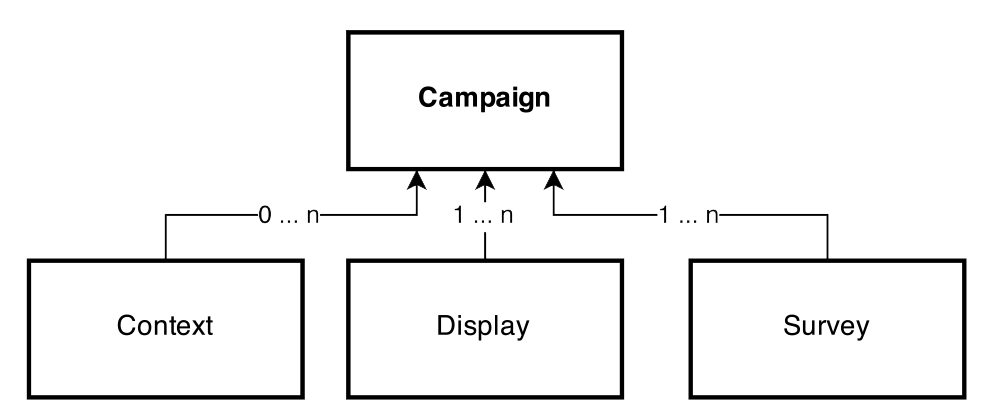
\includegraphics[width=.8\columnwidth]{img/4_implementation/4-dependency-campaign}
    \end{center}
 % \begin{center}\LARGE [BILD]\end{center}
 \caption{Campaign model dependencies}
 \label{fig:4-dependency-campaign}
\end{figure}


++ neue Namensgebung, um in der domain specific language zu bleiben --> application provider / display provider / space provider (anstatt Operator). Wir werden aber nur mit dem Application Provider (anstatt Operator) im System arbeiten





\subsubsection{REST interface}

Defining the REST API. 

% TODO: Explain why I chose which level of separation / detail.

Notes from before I started writing: 
\begin{enumerate}
\item Think about using a Extreme Programming approach http://www.extremeprogramming.org/rules.html
\end{enumerate}
\label{sec:implementation:modeling}

Modeling
	Software Model
	+ Dependencies in between them
	Users
	User Stories
	REST API



\subsection{Prestudy}

First feedback regarding the platform, before launching it. Either I will use this section, or I will make the expert interview (see section \ref{sec:expert-interview}).



\subsection{Not sure about...}

	\begin{enumerate}

	\item \textbf{4.4 Implementation}
		\item leave out!!
		\item these aspets are all part of the MKDOCS documentation inside the repository!

	\item \textbf{Maybe:}
		\item challenges		>> for presentation
		\item problems		>> presentation or docu
		\item frameworks 		>> documentation
		\item deployment		>> documentation

	\end{enumerate}


    

\subsection{PDSurvey Platform}

	The public display survey (\textit{PDSurvey}) platform aims to facilitate the execution and evaluation of surveys on and for public displays. 
	The interactive survey platform, which can be embedded directly onto public displays and be used as a direct feedback channel from inside another application, can be split into three main parts: PDAdmin, PDServer, and PDClient (see figure \ref{fig:4-pdsurvey-platform}). \textit{PDAdmin} contains the administrative interface, allowing display providers to configure questionnaires for their public displays. \textit{PDServer} accommodates the REST service, the persistence layer, and the majority of the application logic. \textit{PDClient} is a web-based interface, containing one possibility for responding to the deployed surveys. 
	The code base of all three parts is deliberately separated from each other, allowing the independent refinement and less dependence between the frontend, the backend, and the server.

	\begin{figure}[btph]
	    \begin{center}
	        % 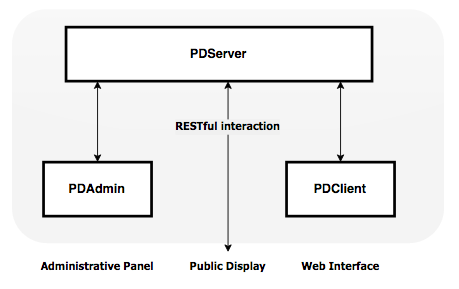
\includegraphics[width=.7\columnwidth]{img/4_implementation/4-overview}
	        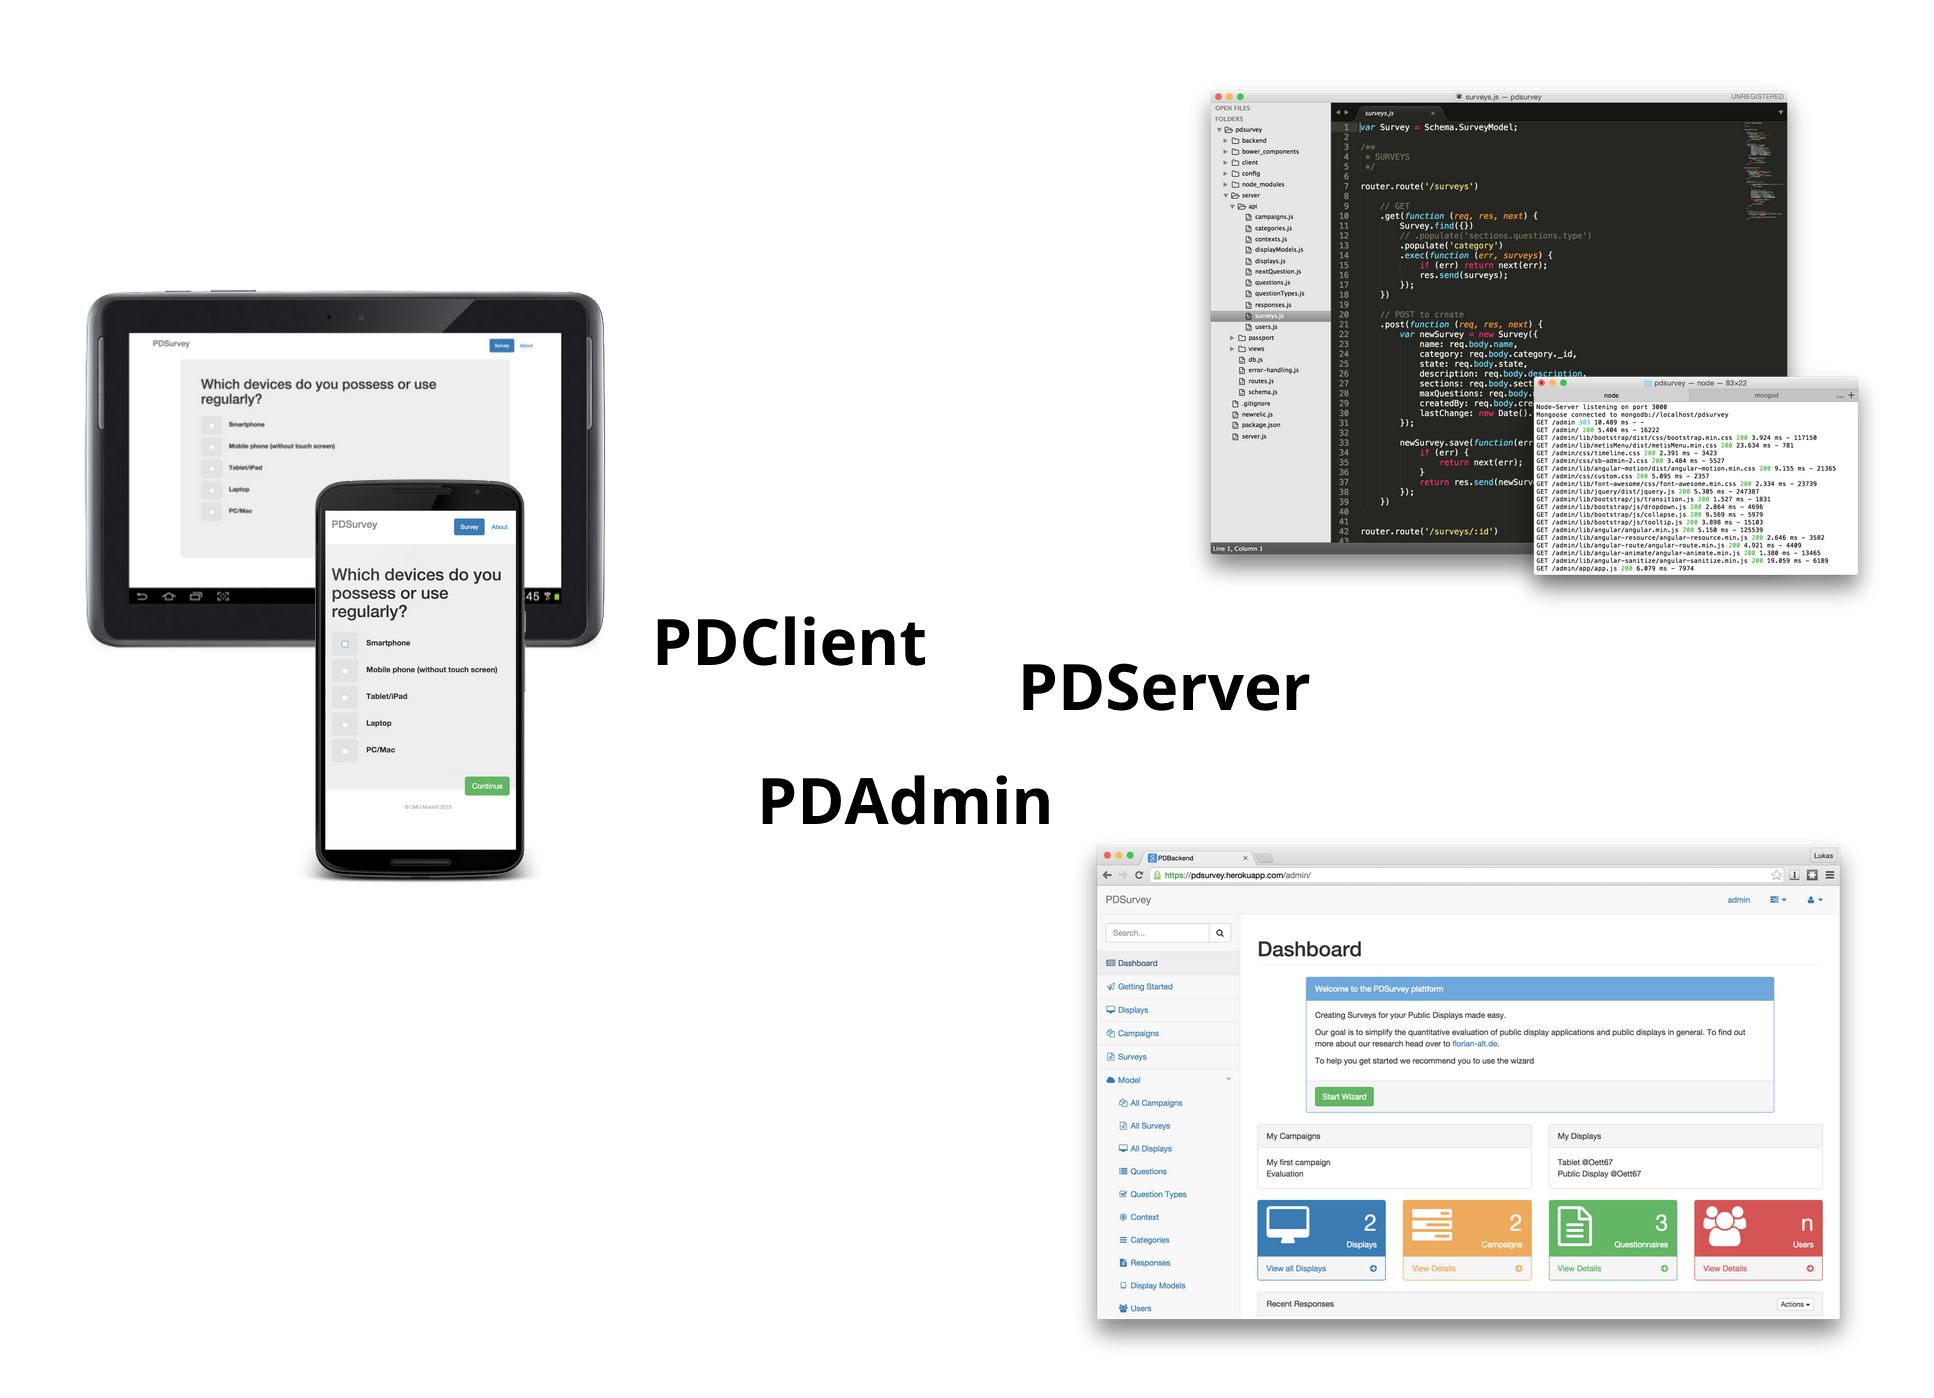
\includegraphics[width=.7\columnwidth]{img/screenshots/pdsurvey-overview/pdsurvey-platform.png}
	    \end{center}
	 \caption[Overview of the PDSurvey platform]{Overview of the PDSurvey platform: (a) PDServer containing the Node.js server, (b) PDBackend is the entry point for administrators and (c) PDClient the interface included on public displays and optimized for mobile devices.}
	 \label{fig:4-pdsurvey-platform}
	\end{figure}



	\subsubsection{PDAdmin}

		For administrative purposes an admin interface was created, enabling display providers to create, manage and distribute surveys to public displays. Display providers have the ability to create their own questionnaires or to select from a list of standardized questionnaires (chapter \ref{chapter:literature-evaluation}).
		The entry point for PDAdmin is the dashboard (see figure \ref{fig:pdadmin-dashobard}). There users get an overview of all relevant information such as how their campaigns are running, and how many responses have been submitted already. 
		% Wizard
		For new users, who haven't created any campaigns, questionnaires or displays yet, the \textit{Wizard} (see figure \ref{fig:pdadmin-wizard}) will be the best place to get started with the survey platform. Users get guided through the creation process of campaigns step by step.
		% Experts
		For more experienced users the navigation options \textit{Displays}, \textit{Campaigns}, and \textit{Surveys} are more advisable. 
		% Admins
		Administrators of the survey platform additionally have the ability to add new \textit{Users}, \textit{Question Types}, or research \textit{Categories}.


	\begin{figure}%[btph]
	    \begin{center}
	        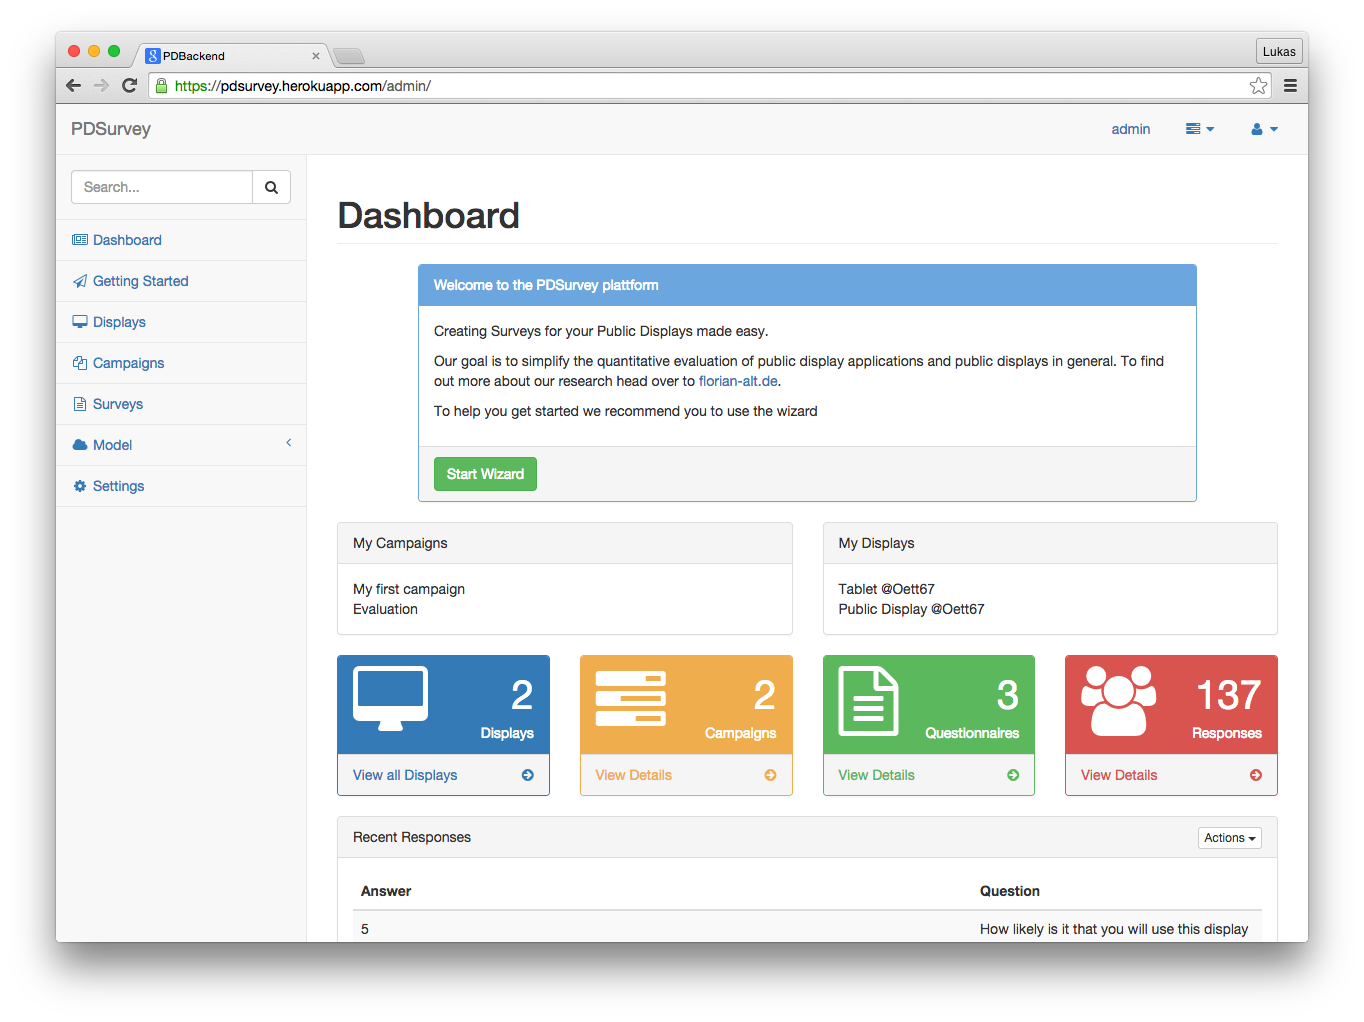
\includegraphics[width=.8\columnwidth]{img/screenshots/pdadmin/dashboard.png}
	    \end{center}
	 \caption[PDAdmin Dashboard]{Dashboard of PDAdmin}
	 \label{fig:pdadmin-dashobard}
	\end{figure}

	\begin{figure}%[btph]
	    \begin{center}
	        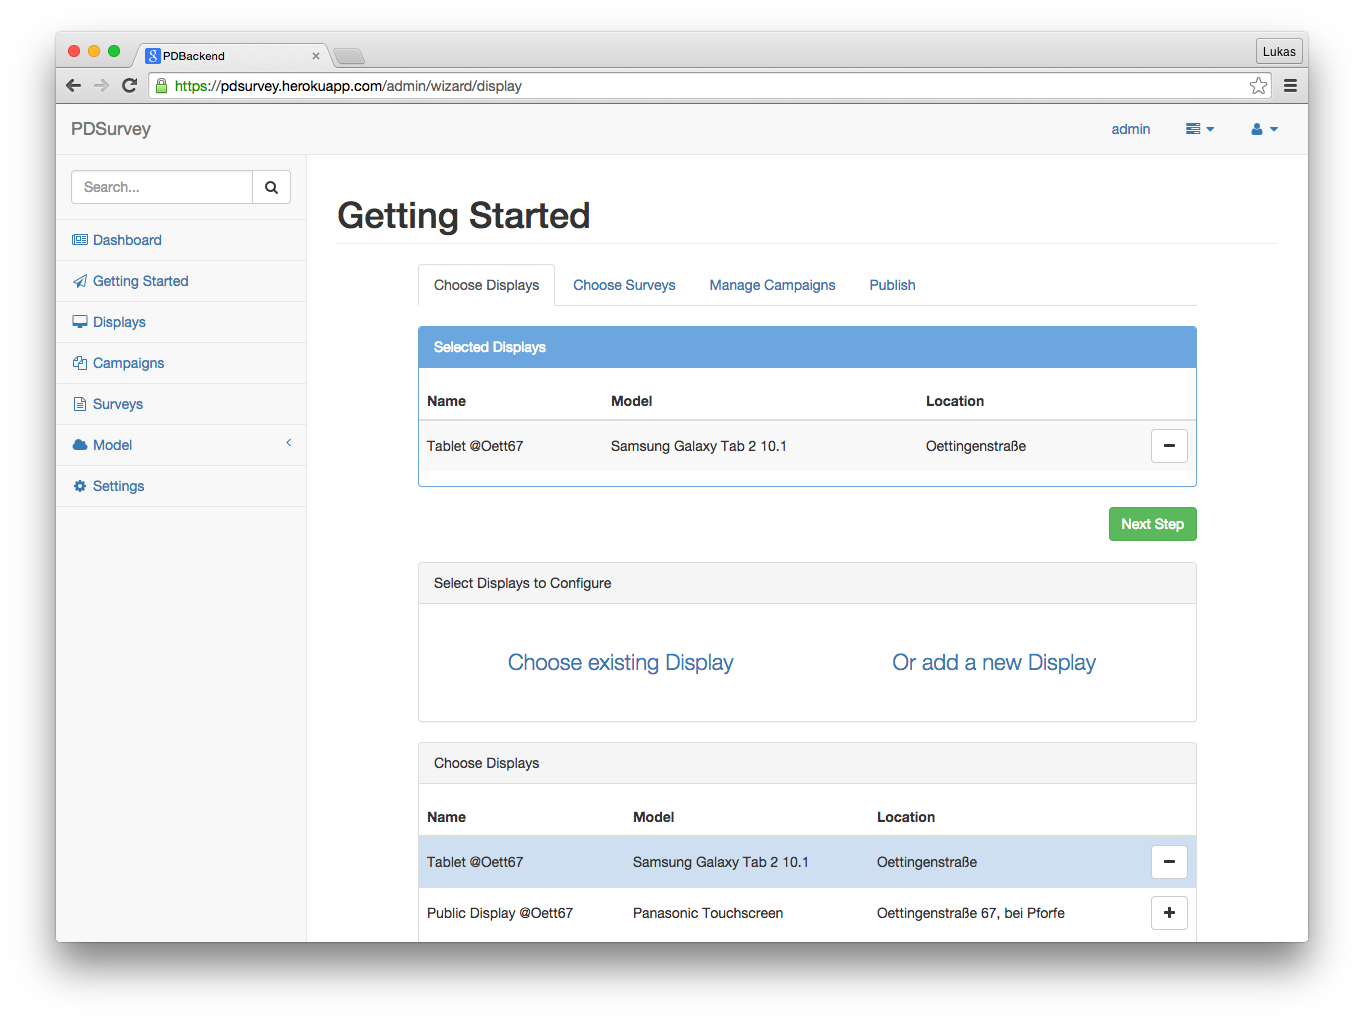
\includegraphics[width=.8\columnwidth]{img/screenshots/pdadmin/wizard-display_selected.png}
	    \end{center}
	 \caption[PDAdmin Wizard]{Wizard for PDAdmin}
	 \label{fig:pdadmin-wizard}
	\end{figure}




	\subsubsection{PDServer}

		The server was written in Node.js and to the outside only offers a RESTful API. All interactions users or developers make with the server are HTTP calls. When performing CRUD operations, all REST calls need to be executed and JSON objects are returned.
		Besides this REST functionality a rudimentary authentication mechanism is already implemented on the server and the capability for further logic, determining which client should ask which question next. This functionality might become of interest when trying to spread standardized questionnaires of longer length across multiple users or multiple displays. It would be intended for the server to keep track which questions have already been answered and to tell each instance of PDClient which question to ask next, in order to achieve a balanced question profile.
		The specification of PDServer's REST API can be found on GitHub\footnote{\url{https://github.com/lukasziegler/masterarbeit/tree/master/docs} (last accessed on April 15, 2015)} and on the enclosed CD (see Appendix \ref{appendix:cd-contents}).



	\subsubsection{PDClient}

		Our client tool was kept as simple and minimalistic as possible. The only communication between PDClient and PDAdmin is via REST calls, exchanging JSON objects. Even though both PDClient and PDAdmin are developed using Javascript frameworks, they have a separate code base. Reasons for this were on the one hand reduction of the application size, on the other hand different requirements of the client version and the administrator panel. PDClient needs to be highly scalable and offer a low latency and fast response time. For PDAdmin it is more important to offer a better usability and a more visual appealing presentation of the results. The goal is to reduce logic and complexity on client-side. Currently PDClient loads all questions for the questionnaire at startup and caches them for later access. 

		% Overview of elements
		PDClient has three main components (see figure \ref{fig:pdclient-screenshots}). The principal part is the \textit{Survey page}. All questions are loaded at once on startup. Then one question gets displayed at a time. Settings for the survey can be modified from PDBackend (e.g. number of questions to display and duration of the survey). Once the user makes a choice, it is directly logged on the server. In a case when a participant aborts answering the survey, the questions answered so far are still recorded. The \textit{About page} was added, since some employees from university said they were skeptical and had doubts regarding the research project, when there is no information whatsoever about which information is logged. To motivate people to participate, a \textit{Welcome page} was added. It turned out that a significantly larger number of people were willing to participate in a survey, after finding out that it will only take one minute, the research is university-related and that it will be used for a Master's thesis.


		\begin{figure}
		    \centering
		    \begin{subfigure}[b]{0.6\textwidth}
		        \centering
		        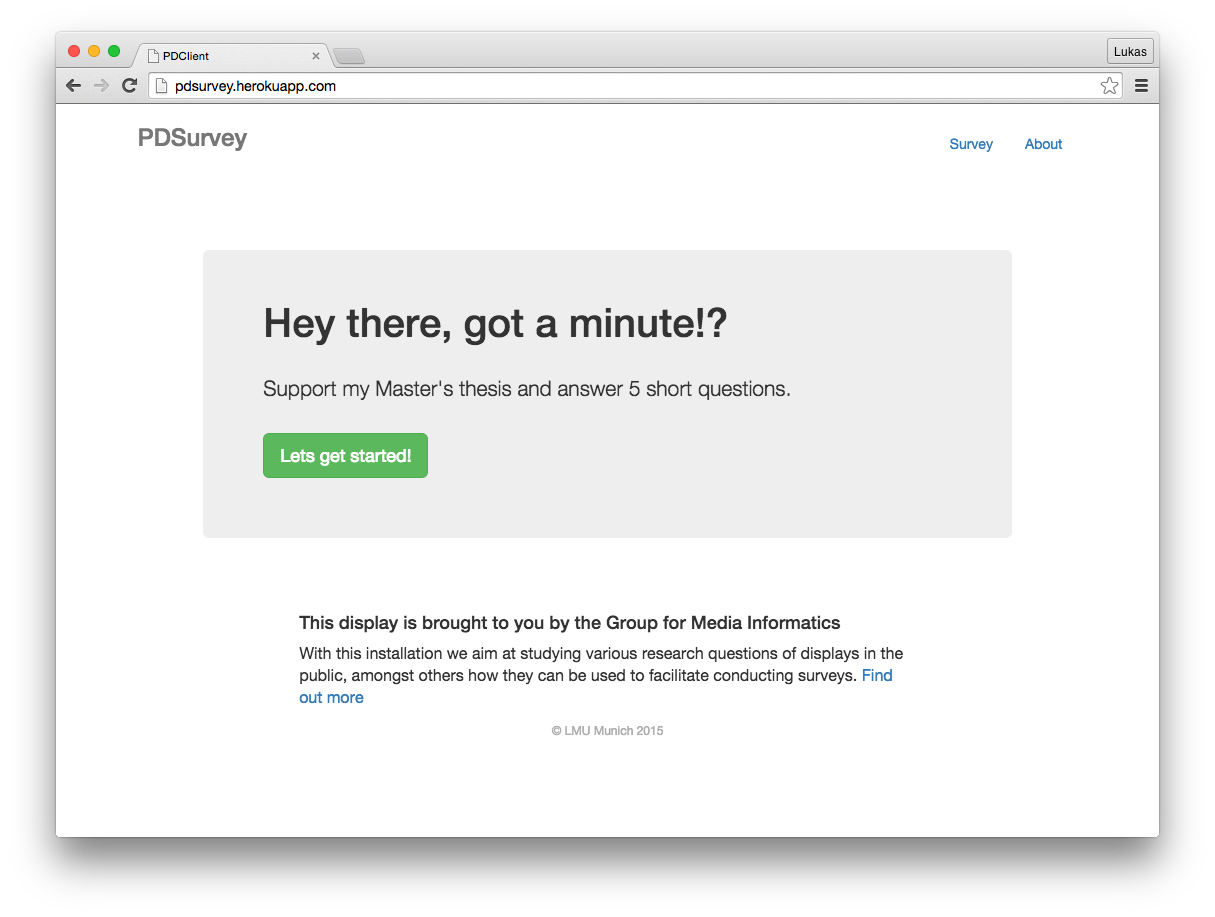
\includegraphics[width=\textwidth]{img/screenshots/pdclient/welcome}
		        \caption{Welcome Page}
		        \label{fig:4-pdclient-welcome}
		    \end{subfigure}
		    \hfill
		    \begin{subfigure}[b]{0.6\textwidth}
		        \centering
		        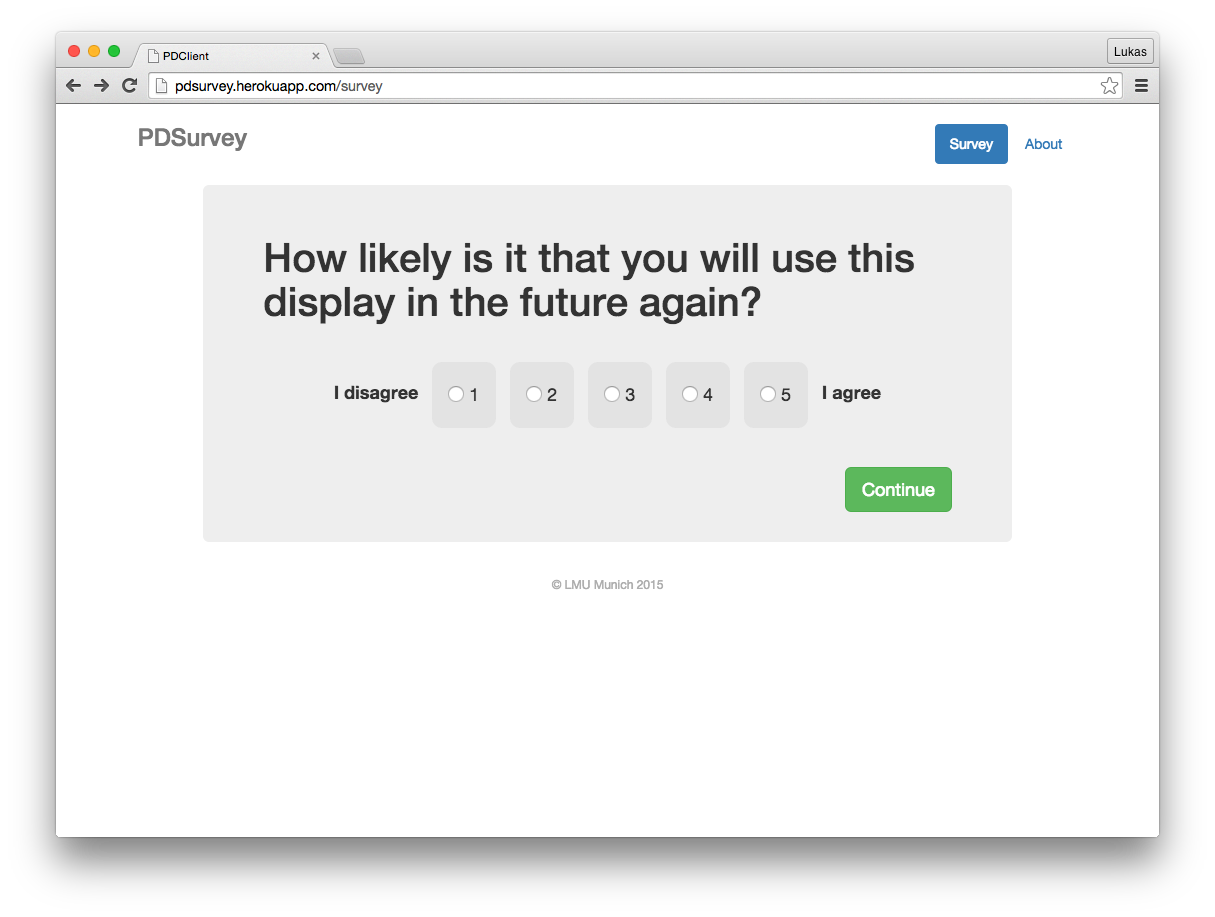
\includegraphics[width=\textwidth]{img/screenshots/pdclient/survey}
		        \caption{Survey page}
		        \label{fig:4-pdclient-survey}
		    \end{subfigure}
		    \hfill
		    \begin{subfigure}[b]{0.6\textwidth}
		        \centering
		        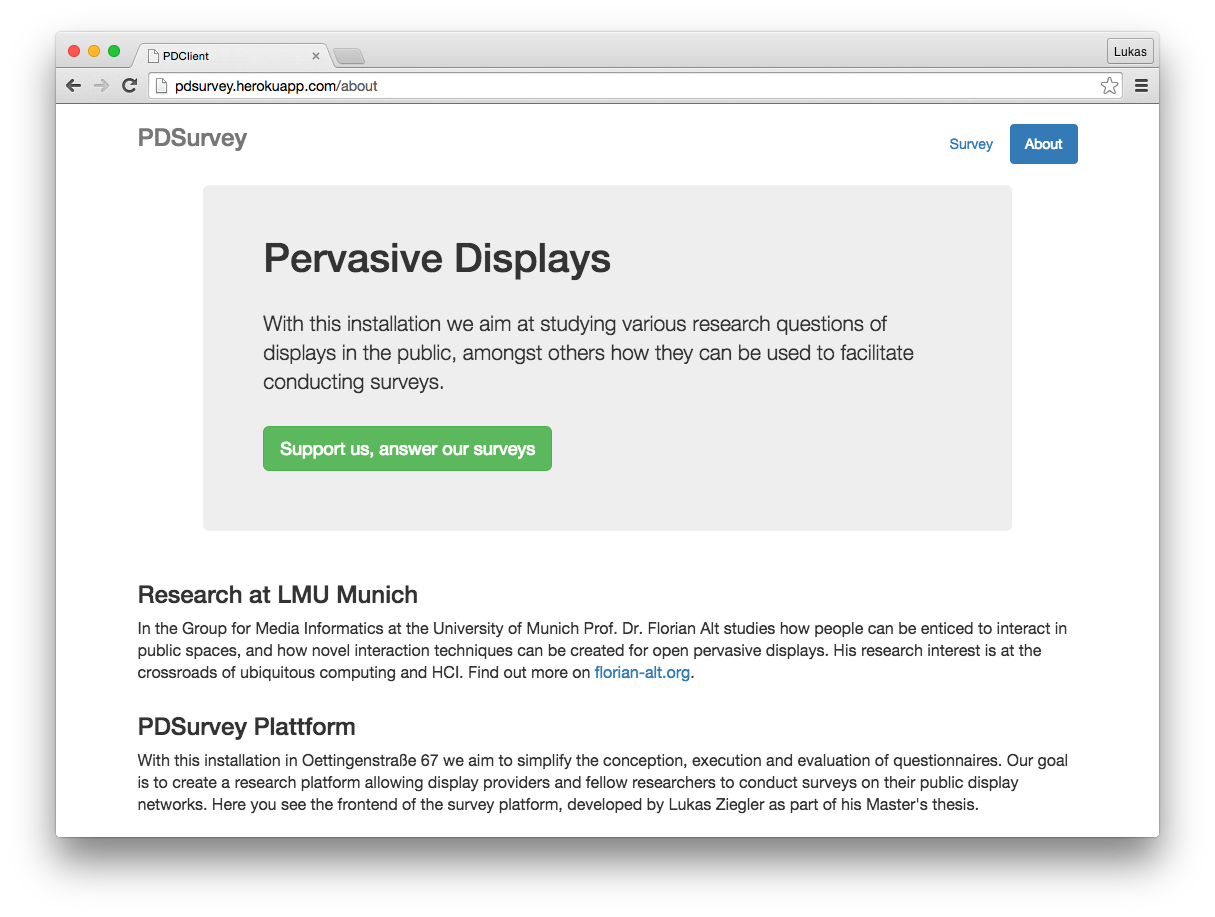
\includegraphics[width=\textwidth]{img/screenshots/pdclient/about}
		        \caption{About page}
		        \label{fig:4-pdclient-about}
		    \end{subfigure}
		    \caption{Overview of PDClient}
		    \label{fig:pdclient-screenshots}
		\end{figure}



	\subsubsection{EmbedCode}

		Offering an embed code for surveys, turned out to be a pure proof-of-concept. The problem was that the Balloon Shooter game, on which \textit{PDSurvey} should be integrated, did not support any HTTP calls or overlays. Thus, we had to fall back on another solution. This embed code was intended to be used by display operators, wanting to include questionnaires hovering over their web-based public display applications. The technical realization was inspired by Web Bug \footnote{\url{http://en.wikipedia.org/wiki/Web_bug} (last accessed on November 26, 2014)}, and the embed code offered by Google Analytics\footnote{\url{https://developers.google.com/analytics/resources/concepts/gaConceptsTrackingOverview} (last accessed on November 26, 2014)}.

		% Implementation
		One minified line of JavaScript code needs to be added before the closing HTML <body>-tag. This minified line creates a <script>-tag in the the Document Object Model (DOM) of the HTML page, injecting a JavaScript file from the \textit{PDSurvey} platform. This personalized scripts first loads jQuery and/or Angular.js asynchronously, creates another instance of PDClient inside of the primary website's DOM. All questions for the questionnaire get loaded via PDServer's RESTful API and the responses get sent back to the server for logging. To avoid conflicts caused through the code injection, all classes and files are prefixed with a unique namespace.






%\________________________________________________________

\cleardoublepage

    \section{Field Study}
\label{chapter:field-study}


	The field study took place during the first two weeks of March, from 3/3/2015 to 3/15/2015 in Oettingenstrasse 67, a faculty building of Ludwig-Maximilians-Universit\"at M\"unchen. Data was collected from the display setup on 14 consecutive days and 28 semi-structured interviews were carried out on five working days during the same two weeks. A total of 117 interactions were registered with the public display installation and 57 survey responses were recorded.

	The goal of this study was to validate our research questions, and to see how users respond to questionnaires being conducted on public displays. We chose to conduct a descriptive study, with a focus on ecological validity, since our research prototype is still in an early stage of development. 




\subsection{Research Questions}

	% MOTIVATE: Why did we bother to do this study?
	One of the main reasons why we conducted this field study, was to get a better understanding of our assumptions and to see how users react to questionnaires on displays in public. Besides, it was of importance to conduct a study ``in the wild'', because there often is a discrepancy between lab studies and field studies. This phenomena has been discussed by Ojala and Kostakos in 2011: ``The first important conclusion we have arrived at is that there exists a huge difference between results obtained in a lab and in the wild using the exact same configuration''\cite{Ojala2011}.

	% What do we assume  /  What do we want to know
	One hypothesis we made for the development of our first research prototype of the \textit{PDSurvey} platform was that we can simplify the process of conducting and deploying surveys to large public display networks. Since this is a rather large claim, we broke down this hypothesis to the following more fine-grained statements:

	\begin{enumerate}
		\item Which feedback channels are best suited for completing surveys in public?
		\item Why did users approach the display? What motivates them to fill in surveys in public? 
		\item How did the user notice and perceive the survey on the display?
		\item Which question types are best suited for questionnaires carried out in public? 
	\end{enumerate}

	In addition to these questions we were also interested in user stories, the feedback real-world users gave us in regards to answering surveys on screens in public. For this reason we also conducted semi-structured interviews in parallel to the quantitative evaluation of the \textit{PDSurvey} platform. In order to get as authentic and personal feedback as possible, we stuck loosely to the designated questions of the semi-structured interview (see Appendix \ref{appendix:interviews}), in order to allow users to also tell us new stories, which we wouldn't have thought of before.

	These research questions were represented in the \textit{PDSurvey} questionnaires and semi-structured interviews. Questions which would go beyond the scope of this thesis, and might serve as follow-up questions for further research, are gathered in chapter \ref{chapter:future-work}, Future Work.




\clearpage
\subsection{Pre-Study}

	Smaller Pre-studies accompanied the development of \textit{PDSurvey} and the related field study, in order to get early feedback in the development process. 
	% PDAdmin
	For the backend it was good to find out more about the ...


	\begin{enumerate}
	\item intrinsic motivation
	\item adjusted font-size for large / small screens
	\item Backend: wizard
	\end{enumerate}



	% Adjustments on the day prior to the evaluation
	The day prior to the launch of the actual field study was used for assembly and for last adjustments, like change of font size, adjustment to the position of certain UI elements, and for collecting implicit feedback from users observing but not approaching the display. Only from observing it could be seen that a more effective call-to-action was needed. Many people looked at the display, noticed that something has changed with the setup, but no one started interacting or was willing to complete the questionnaire. Therefore a more catchy start screen was introduced for the tablet (see \ref{fig:5-pdclient-intro}) and the option panel of the TV screen was also modified \ref{screenshot:options}. This observation is very much in line with the self-determination theory by Richard Ryan and Edward Deci \cite{ryan2000self}.


	\begin{figure}
	    \begin{center}
	        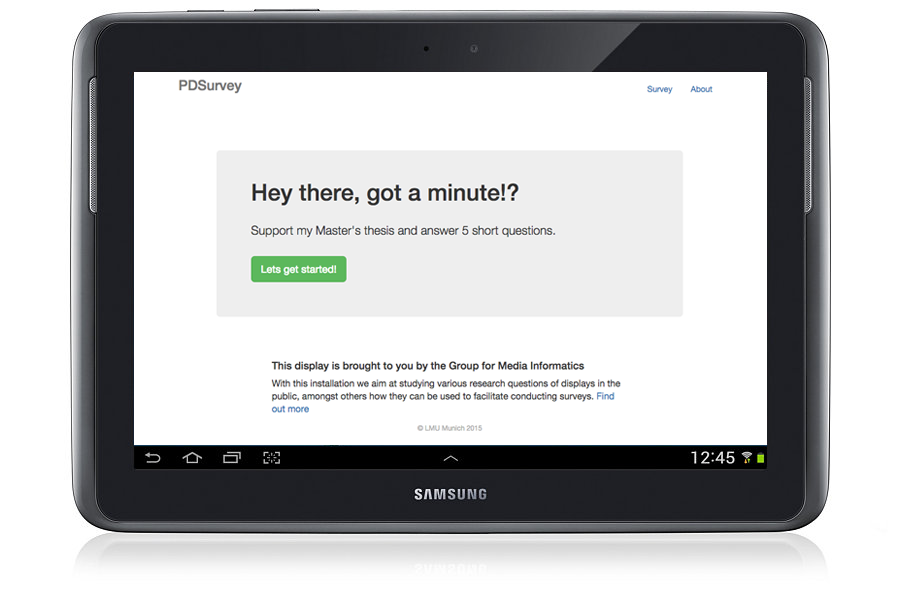
\includegraphics[width=.7\columnwidth]{img/5_field-study/pdclient-startscreen.png}
	    \end{center}
	 \caption{PDClient: Using intrinsic motivation to motivate users to participate in a short questionnaire}
	 \label{fig:5-pdclient-intro}
	\end{figure}
	

	% Intrinsic motivation
	To increase the motivation for users to participate, additional intrinsic motivation was given to increase the response and acceptance rate of the public surveys, as proven by Richard Ryan in his self-determination theory\footnote{http://www.selfdeterminationtheory.org/} \cite{ryan2000self}. We stated that the questionnaire consists of five questions, that it will only take one minute to complete and the results are for a Master's thesis at the university. This information was displayed as a splash screen on the tablet (see figure \ref{fig:5-pdclient-intro}).



	



\clearpage
\subsection{Study}

	% give the reader enough information to replicate the experiment
	We deployed the \textit{PDSurvey} platform to a public display setup, which has already been running since several months in the entrance hall of the faculty building. The public display setup has consistently attracted new and returning users to participate. 
	A descriptive research type was chosen as the study type. Our aim is to describe and observe how users react to the new display setup. Only one study prototype is deployed, without varying any variables. The goal was to get first feedback on how people perceive filling in questionnaires on digital signage in public, before getting into more fine-grained research (see chapter \ref{chapter:future-work}). 
	Both quantitative and qualitative data was collected as part of the field study. Quantitative data was obtained through the \textit{PDSurvey} system and qualitative data was collected through semi-structured interviews.
	The distribution of the preferred feedback channel was logged inside of the Balloon Shooter game (see section \ref{chapter:field-study:apparatus}) and asked in all semi-structured interviews.


	\subsubsection{Design}
	\label{chapter:field-study:design}

	% Goal: Which Feedback Channel
	Our primary goal was to find out which feedback channel users preferred to respond to surveys in public. Each user had the choice to respond to the questionnaire on a TV display (1), on a tablet (2) to the right of the TV screen, via their own smartphone (3) or via email (4). The order of all four feedback options was randomized.
	After completing the Balloon Shooter game on the primary TV screen, each participant was confronted with an options panel (see figure \ref{fig:5-feedback-options}), asking the user to support our research and to respond to a short questionnaire. The feedback channel chosen was logged and the user next had the opportunity to respond to the same questionnaire on all four feedback channels. 
	We displayed the same five questions (see table \ref{table:5-questions-asked}) and chose to limit the number to five questions, to avoid low participation rate and low response rate.

	\begin{figure}
	    \begin{center}
			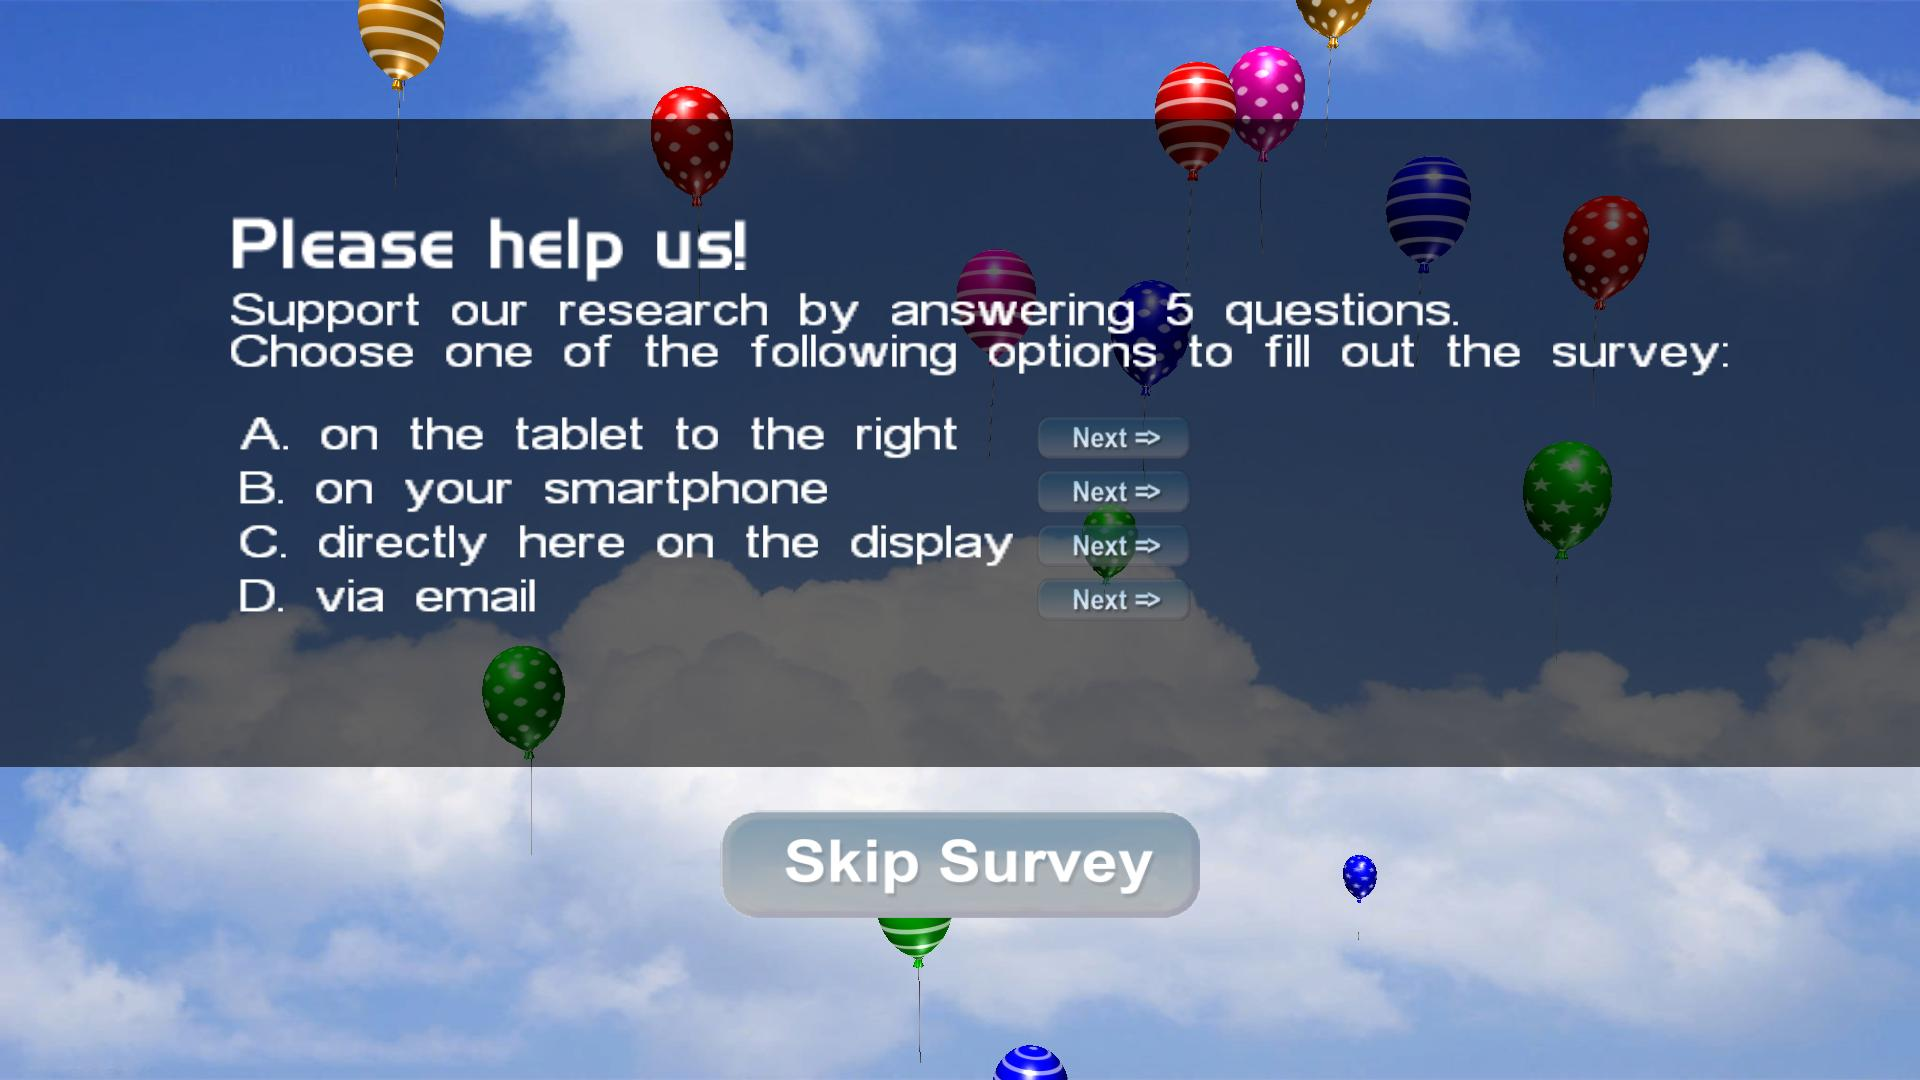
\includegraphics[width=.65\columnwidth]{img/screenshots/balloon-game/options-overview.jpg}
	    \end{center}
	 \caption[Feedback Channel: Option Panel]{Option panel, embedded after a game of Balloon Shooter, promting the user to choose a feedback channel.}
	 \label{fig:5-feedback-options}
	\end{figure}

	% Table: Questions asked on PDClient
	\begin{table}[h]
		\label{table:5-questions-asked}
		\small
		\center
		\begin{tabular}{lc}
\toprule
\textbf{Wording}                                                     & \textbf{Question Type} \\ \midrule
1. How often have you used this display before?                         & Numeric                \\
2. How likely is it that you will use this display in the future again? & 5-point Likert scale   \\
3. Which devices do you possess or use regularly?                       & Multiple choice, 5 options                        \\
4. In which area do you study / work?                                   & Text field             \\
5. What was your motivation for approaching and using this display?     & Text field            \\
\bottomrule
\end{tabular}

		\caption[Questions asked]{Questions asked on all four feedback channels}
	\end{table}

	% I: QUESTIONNAIRE

	% Question Types
	In order to also get first insights into how well certain question types are suited for surveys in public, where a short completion time is crucial, we varied between the following question types and kept them in the same order: numeric questions, Likert scale, multiple choice (based on check boxes) and two text fields for responses of undefined length. 

	% Study setup: pure observation (no indep. variables / conditions)
	Due to the nature of descriptive studies, we only observed the users' behavior and observed how our study setup was used. The parameter of interest was the feedback channel chosen to respond to the survey. Since we didn't vary any conditions, no independent variables are present.

	% II: SEMI-STRUCTURED INTERVIEW

	To find out more about the users' motive for approaching the display setup, we also carried out semi-structured interviews in parallel to the field study of the PDSurvey platform. The goal of the interviews was to get qualitative feedback from all age groups and backgrounds. Getting a better understanding of how people respond to questionnaires in public, helps us improve the \textit{PDSurvey} platform.




	\subsubsection{Participants} % provide the necessary information about the people who took part in your experiment
	\label{chapter:field-study:participants}

		In total 57 questionnaires were submitted and 28 semi-structured interviews were conducted during the two week study period. As for the study size, we took the findings from Alt et al.\cite{Alt2012HowToEvaluate} as a rough guide, for how many participants to include four our study. According to Alt et al. most field studys have an average of 26.9 interviews and 38.4 questionnaire responses.
		Information about the background of the participants was assessed both in the questionnaire and in semi-structured interviews (see table \ref{table:demographics}). Due to the limited number of questions in the questionnaire, only one the age of the participant was asked. In the semi-structured interviews information regarding the participants' age, gender, and working/study area were asked.

		Based on the fourth question (``In which area do you study / work?'') we can draw a conclusion about the study field of the survey participants. As far as indicated all people responding to the \textit{questionnaire} installed on the public display setup were students. Out of 57 responses, 42 could be assigned to a study field. The remaining 12 submissions consisted of responses such as \textit{bavaria, bib, home, munich, muc} or were left empty. The study fields most frequently represented were Computer Science (23,8\%), followed by Political Science (14.3\%), Japanese Studies (11.9\%), and Anthropology (11.9\%), Cultural Science (9.5\%), and Business (9.5\%). Other study fields mentioned were Physics, Sociology, Ethnology, Communication Science, Sports, and Science \& Technology. 

		For the \textit{semi-structured interviews} we collected more detailed information about the participants' background. Out of the 28 participants, 72.4\% were male and 28.6\% were female. The average age was 31 years, with an age distribution ranging from 20 years up to 69 years (median=25, SD=13.2). Due to the wide variety of faculties and a library being located in the same building, various technical backgrounds were present. What they all had in common was their affiliation to LMU Munich, either because of being a student themselves, working at the university or being otherwise related to the university. In total 23 students, three employees, and two retirees were interviewed. The study fields which were most frequently represented are Computer Science (16.7\%), Japanese Studies (16.7\%), Ethnology (12.5\%), and Political Science (12.5\%). Other areas mentioned were Sociology, Communication Science, Law, Physics and Engineering. 
		% Participants vs Passer-by
		Eleven of the 28 interviews were conducted with actual participants of the public display study setup (39.3\%), the remaining 17 interviews (60.7\%) consisted of people passing by the display setup.


		\begin{table}[bh]
			\small
			\center
			\begin{tabular}{lllll}
\toprule
   & \textbf{Participants Of Survey} &  &   & \textbf{People Interviewed}                        \\
   \midrule
10 & Informatics                            &  & 4 & Informatics                                        \\
6  & Political Science                      &  & 4 & Japanology                                         \\
5  & Japanese Studies                       &  & 3 & Ethnology                                          \\
5  & Anthropology                           &  & 3 & Political Science                                  \\
4  & Cultural Science                       &  & 3 & \textit{employees} (PhD, public officer, SysAdmin) \\
4  & Business                               &  & 2 & \textit{in pension}                                \\
2  & Physics                                &  & 1 & Communication Science                              \\
2  & Sociology                              &  & 1 & Sociology                                          \\
1  & Ethnology                              &  & 1 & Law                                                \\
1  & Communication Science                  &  & 1 & Physics                                            \\
1  & Sports                                 &  & 1 & Engineering                                        \\
1  & Science and Technology                 &  &   &               \\
\bottomrule
\end{tabular}

			\caption[Demographics of Field Study]{Demography for the survey data (left) and the semi-structured interview (right).}
			\label{table:demographics}
		\end{table}


		% HOW WE OBTAINED THE PARTICIPANTS
		The selection of participants for the completion of the \textit{questionnaire} was not influenced by us. All survey responses were made in their own interest, no reward was given for participating in this ``in the wild''-study.
		The selection of the participants for the \textit{semi-structured interviews} was influenced by how users reacted to the display setup. Our primary goal was to observe and interview active users of the public display setup, in order to get a better understanding of how they perceived the setup and to get insights into which feedback channel they chose why. In order to also understand why people did not approach, or if they have any concerns, people passing by were also interviewed. 
		
		Before starting the semi-structured interviews, all people participating were asked whether they had already noticed the display setup and/or the option to fill in a survey. 
		This allowed us consider the novelty effect for evaluation and to differentiate between three groups: participants who approached the display by themselves (and were observed doing so), people passing by the display (noticing the display, however not approaching it) and the last group of people simply passing by (not having noticed the display). The distribution between the groups was as follows: 11 active participants, 14 passerby (who have noticed the displays before), and 3 passerby (who saw the display setup for the first time). 

		Out of all people passing by no one has noticed the option to fill in a survey. Out of the active participants, 5 out of 11 have noticed the option to respond to a survey on different channels.
		To increase the amount of feedback, we approached people from all three groups. The number of survey responses was not artificially increased by asking passersby was.
		



	\subsubsection{Apparatus}
	\label{chapter:field-study:apparatus}
		% give details of any equipment used, including thinkgs like questionnaires and other tests

		The permanent setup consisted of a 55-inch touch-sensitive TV screen, connected to a laptop running on Windows 7, and a Samsung Galaxy Tab 10.1 tablet positioned to the right of the TV screen on a console. The TV screen was positioned on a 60cm high stand, resulting in a positioning at eye level. The tablet was placed on and fixed to a conductor's stand to the right of the TV screen (see figure \ref{fig:5-study-setup}). Our object of investigation was the TV screen with touch support, running an interactive game called \textit{Balloon Shooter}, developed by Jiamin Shi. After users completed the game, they were asked via a prompt to fill in a questionnaire on one of the four provided feedback channels (see figure \ref{fig:5-feedback-options}). The courtesy for the Balloon Shooter game and the survey implementation on the TV screen goes to Jiamin Shi.

		\begin{figure}
		    \begin{center}
   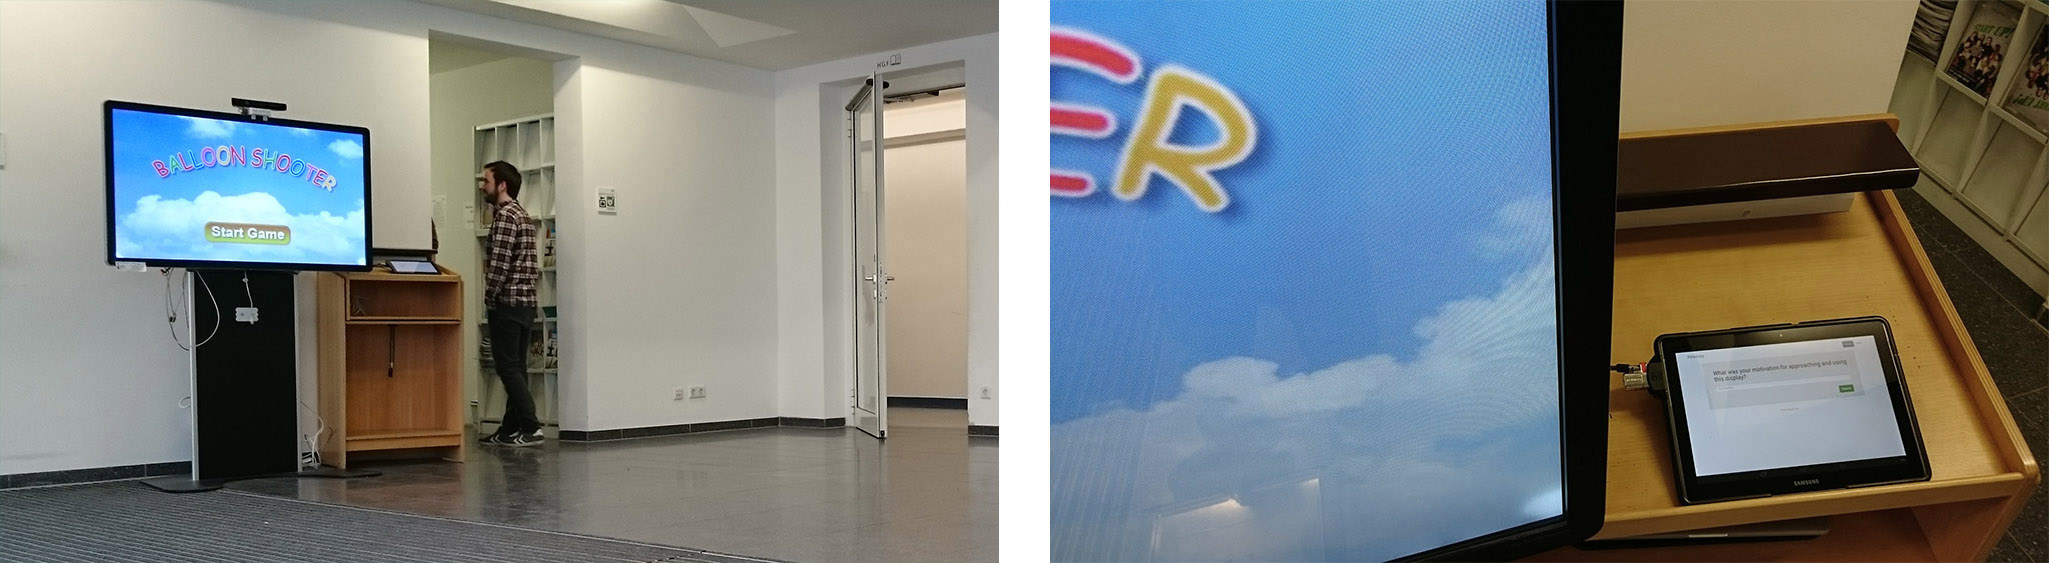
\includegraphics[width=\columnwidth]{img/5_field-study/study-setup.jpg}
		    \end{center}
		 \caption{Overview of the study setup in the entrance hall of the faculty building.}
		 \label{fig:5-study-setup}
		\end{figure}

		Each user had the opportunity to respond to the \textit{questionnaire} either directly on the TV screen (1), on the tablet to the right of the big TV (2), via their own smartphone (3) or via email (4). The first option was embedded natively into the Balloon Shooter game, offering a consistent UI and the most direct feedback channel. When choosing the tablet as an option, users were prompted to move to the right and to answer five questions on the tablet. The Android tablet was running KioWare Lite\footnote{\url{http://www.kioware.com/android.aspx} (last accessed on April 21, 2015)}, a kiosk app for Android, and displaying the responsive frontend of PDClient for the entire time of the study. Choosing the third option prompted the user to either scan a QR code with their smartphone or to open a URL\footnote{\url{https://pdsurvey.herokuapp.com/} (last accessed on April 21, 2015)} in their mobile browser. The last option consisted of an input field embedded into the Balloon Shooter game on the TV screen, asking the user to enter their email address. The address was logged to a txt-file, which was scanned every 5 minutes by the Windows task scheduler. An email reminder was sent to the user with a request to complete the survey. For sending the email from the TV screen, a Python script\footnote{\url{https://github.com/lukasziegler/python-send-mail} (accessed on March 15, 2015)} was written, using a modified version of TLS authentication in order to comply with the university's SMTP server. Screenshots of all four options can be found in Appendix \ref{appendix:screenshots-balloon-shooter} on page \pageref{appendix:screenshots-balloon-shooter}.
		% What was logged
		For the permanent setup the following data was logged: the timestamp of the users choice, which feedback channel the user chose to respond to the survey, and whether they skipped the call to participate in the survey or if they stopped playing the game (determined via timeout). 
		% Questionnaire used
		On all four feedback channels a self-made questionnaire was used, since the focus was on finding which channels and question types are best suited in general for being used on public display. This was the reason why we did not use any of the standardized questionnaires mentioned in chapter \ref{chapter:literature-evaluation}. 

		% II) SEMI STRUCTURED INTERVIEW
		For conducting the \textit{semi-structured interviews}, two questionnaires were used as a rough guidance, one for participants, and one for passerby. A voice-recorder (smartphone) was used additionally to record the interviews, to be able transcribe and code all of conducted interviews. Each semi-structured interview loosely followed the outline presented on page \pageref{appendix:semi-structured-interview}. Audio recordings and transcriptions are on the attached CD.
		% III) BALLOON SHOOTER GAME
		The main application installed on the public display was a game called \textit{Balloon Shooter} developed and run by Jiamin Shi, a PhD student at the Group for Media Informatics at LMU Munich. It was first installed on January 7th 2015 and has been running in different versions since then. Public audience was already used to it for roughly two months and adapted to it well. In 2,5 weeks in February\footnote{Based on the evaluation of log data from 05/02/2015 to 23/02/2015, reported by Jiamin Shi.} usage statistics reported that the game was played a total of 305 times.



	\subsubsection{Location}

		All parts of the field study were carried out in Oettingenstrasse 67, the faculty building for Computer Science of Ludwig-Maximilians-Universit\"at M\"unchen. In the same building research institutes for Ethnology, Political Science, Japanese Studies, and Physics are also located. The study was carried out in the entrance hall of the university building. Figure \ref{fig:5-entrance-hall} gives an overview of the entrance hall and of the paths most people take while crossing the room. The excerpt is based on the universities floor plan\footnote{\url{http://www.uni-muenchen.de/funktionen/gebaeudeplaene/7070_d_00.pdf} (last accessed on March 22, 2015)}, and was inspired by Sandra Zollner \cite{zollner2014thesis}. For her bachelor's thesis she conducted a study in the same location one year ago and analyzed the visitor flow. According to Zollner ``approximately 59\% of all passers-by used path 1'' to get something from the lockers or to leave through the door to the library. 28\% of the people were taking path 2 and 13\% were taking path 3.
		% My observations
		In our field study it was also evident that the majority of the visitors took path 1. This group usually was fairly target-orientated, or in a hurry. Otherwise, on days with bad weather, people had their break in the entrance hall, or waited for someone. On days with good weather people usually took their breaks outside and only passed through the entrance hall, coming from the library, picking up something from the locker room and going outside.

		\begin{figure}[hb]
		    \begin{center}
		     \fbox{	
		     	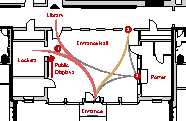
\includegraphics[width=.7\columnwidth]{img/5_field-study/entrance-hall.pdf}
		     }
		    \end{center}
			 \caption[Floor Map of Entrance Hall]{Floor map of the entrance hall, where the field study was carried out. User paths, and the surrounding environment including facilities such as the library can be seen.}
			 \label{fig:5-entrance-hall}
		\end{figure}




	\subsubsection{Procedure}
		% tell the reader how the study was carried out in practice

		All participants of the semi-structured interview were asked a similar set of questions (see Appendix \ref{appendix:interviews}). Based on the group they belonged to, either questionnaire 1 (for participants of the display setup) or questionnaire 2 (for passersby) was chosen. In order to speed up the interviewing process and to get away from a plain question-response schema, the questions on the printed out questionnaire only survey as a rough guideline. 

		% Instructions given
		For people having trouble understanding the concept of the public display installation, the situation was described as follows. ``Imagine you are in a shopping mall or at an airport using one of those large displays to find some information. After having found what you were looking for, you get asked to answer a short questionnaire. How would you react to it?'' A full transcription of all questions and responses can also be found on the enclosed CD. 

		The participants for the PDSurvey questionnaire were not additionally motivated. All they saw was the options panel after completing the Balloon Shooter game (see figure \ref{fig:5-feedback-options}) or the welcome screen of the tablet (see figure \ref{fig:5-pdclient-intro}) while passing through the entrance hall. A complete copy of what the users were able to interact with, can be seen on the attached CD (see Appendix \ref{appendix:cd-contents}).


		% REMINDER: only give RELEVANT information to the reader!
		% > only provide details if they are needed for replication
		% > or if they are relevant to the outcome of the experiment



\clearpage
\subsection{Results}

%%% QUANTITATIVE DATA %%% = pure facts
  % just tell the reader what you found

	We received a total of 57 filled in surveys, submitted via all four of the provided feedback channels, and carried out 28 semi-structured interviews. No treatments were applied to the dataset, descriptive statistics will follow bellow. The presentation of the evaluation is divided into three parts. First we will have a look at which feedback channel is most popular, followed by the quantitative results of the PDSurvey questionnaire, and concluded with the results from the semi-structured interview. 


% I) Descriptive Statistics
% - provide summaries of group performance
% - present: average, mean, mode
% - describes: standard deviation, range (how it is spread)
% - describes: frequency of data (if relevant)

% presentation of data
% - don't present data multiple times
% - either use a TABLE or a GRAPH
% - always explain to the reader in words what the results show
% - tables / graphs should be self explanatory
% - the text should be comprehensible without taking a look at the figures




	\subsubsection{Feedback Channels}
	\label{5:results:feedback-channels}

	The preferred feedback channel was determined in three ways. First, based on the log file from the options panel of the TV screen (see figure \ref{fig:5-feedback-options}). Second, based on the interview responses. And third, by analyzing all of the logged questionnaire responses made on all four feedback channels. The third way, however, has to be treated with caution, since it evaluates all logged responses, which is prone to distortions.

	% PREFERRED CHANNEL
	For the first way, users had the option to choose one of the four offered feedback channels through a selection on the large TV screen. Based on this log data of the TV screen, a good comparison of the feedback channels can be made, since all direct responses made on the tablet are excluded from this summary. The most popular feedback channel was the tablet (46.15\%), followed by the TV screen (30.77\%), smartphone (15.38\%), and email (7.69\%).
	% based on Interviews
	In order to have another source of input, the same question was asked at the end of every semi-structured interview. Based on this quantitative data from the interviews the response via tablet (42.86\%) was most popular again, followed by the TV screen (32.14\%). Interestingly, for the interview data the option to respond via email (17.86\%) is more popular than smartphone (7.14\%). 
	

	\begin{table}[h]
		\small
		\center
		\begin{table}[h]
\center
\begin{tabular}{lllll}
\multicolumn{2}{l}{\textbf{From Survey Data}} &  & \multicolumn{2}{l}{\textbf{From Interviews}} \\
30.8\%                   & \multicolumn{3}{l}{on public display}      & 32.1\%                  \\
46.1\%                   & \multicolumn{3}{l}{on tablet}              & 42.9\%                  \\
15.4\%                   & \multicolumn{3}{l}{on smartphone}          & 7.1\%                   \\
7.7\%                    & \multicolumn{3}{l}{at home / via email}    & 17.9\%                 
\end{tabular}
\caption[Feedback Channel]{Preferred feedback channel for answering surveys.}
\label{table:5-feedback-channel}
\end{table}
		\caption[Feedback Channel]{Preferred feedback channel for answering surveys.}
		\label{table:5-feedback-channel}
	\end{table}


	% LOG data / little bit distorted ...
	When evaluating all logged responses, the same sequence can be seen. The majority of the surveys were completed through the tablet, followed by the TV screen, smartphone, and email. The ratio, however, is highly distorted for this scenario. This is due to the tablets sole purpose to be used to fill in surveys in our setup, and the additional intrinsic motivation given directly on the tablet's start screen (see section \ref{chapter:field-study:design}). The following ratio has to be treated with caution. In total 57 responses were made on all four feedback channels, 50 originated directly from the tablet (87.72\%). Four responses were recorded on the TV screen (7.02\%), two via smartphone (3.51\%), and one via email (1.75\%). Since this listing only contains the number of responses, it should not be taken as a base for the comparison of the feedback channels' popularity. %% = interpretation! 
	For a comparison of the \textbf{feedback channels} the log data from the option panel and the responses of the semi-structured interviews are more suitable (see table \ref{table:5-feedback-channel}).




	\subsubsection{Survey Responses}
	\label{5:results:survey}
	%% Evaluation of all five questions

	Next, the evaluation of all responses made to the questionnaire will follow. In total, five questions were asked on each feedback channel and 57 responses logged. Three times the response was canceled after the first question, once after the second question, four times after the third questions, the remaining 49 responses were complete.

	% 1) How OFTEN have the users USED this display BEFORE?
	The first question (\textit{How often have you used this display before?}) was measured as a numeric response. People have on average used the display 6.9 times before. For 25 people (43.9\%) of the users it was the first time using the display setup, 11 people (19.3\%) have used it once before, 18 people (31.6\%) between two and ten times, and the remaining 3 people (5.2\%) more than ten times.
	% 2) How LIKELY is it that you will USE THIS DEVICE AGAIN?
	For the second question (\textit{How likely is it that you will use this display in the future again?}), based on a 5-point Likert scale, the response was fairly uniformly distributed (average=3.04, SD=1.46). The whole scale from 1 (not likely at all) to 5 (very likely) was represented. No clear trend could be seen. When only considering the responses collected from the large TV screen, a better perception can be noticed. There, the responses to this question had an average of 4.5 (SD=0.866), showing a trend towards a positive perception of the large display setup. However, due to the low number of responses for the TV display (only 4 responses), this conclusion can not be regraded as significant. 
	% 3) DEVICES the users possess
	Taking a look at the devices users possess might give us first insights into why users chose which feedback channel (\textit{Which devices do you possess or use regularly?}). Overall, the majority of the people participating in the survey already owned a smartphone (79.3\%). The second most popular response was laptop (73.6\%), followed by tablet (41.5\%), and desktop computer (26.4\%). Still, 18.9\% of the users indicated that they possess a feature phone and use it regularly. On average each participant possessed 2.4 devices. 
	When looking at which combinations of devices were most frequent, twelve people responded that they own a smartphone, tablet, and laptop. Twelve other people indicated that they possess a smartphone and laptop. Six people own a smartphone, laptop, and desktop.
	% 4) Study area >> demographics
	The fourth question (\textit{In which area do you study / work?}) was used to get a little insight into the background of the survey users. Only the occupation of each participant can be derived from the questionnaire. For a full evaluation of the demographic background of all participants, refer to section \ref{chapter:field-study:participants}.
	% 5) REASONS FOR APPROACHING
	The last question (\textit{What was your motivation for approaching and using this display?}) collected the main resons why people have approached the display setup. The main reasons mentioned were ``curiosity'' (12x), ``fun'' (10x), ``boredom'' (8x), ``interest'' (2x), and ``during breaks'' (2x). Other reasons mentioned were ``it is there, so why not?'', ``it is there and colourful'', or ``I've never seen it before in this spot, wanted to know what it is about''.




	\subsubsection{Interview Responses}
	%% INTERVIEW DATA (a combination of facts + evaluation)

	The evaluation of the semi-structured interviews was based on Grounded Theory \cite{strauss1990basics}, promoting a systematic evaluation of the interview transcripts.
	% ANY INTERFERENCES
	To avoid any interferences between the two groups of people who have already participated in the study setup and people passing by. Each passerby was asked, before starting the interview, whether he has noticed the public display setup, and whether he has already interacted with the installation. Out of all passerby no one has previously been interacting with the game or survey platform. 82.4\% (14 of 17) of the passerby have already noticed the public display installation before. However, none of the passerby has previously participated in the game. The remaining 17.6\% have neither approached the display nor noticed it previous to the interview. 


	% I) REASONS mentioned for choice of feedback channel
	% > TV Screen
	The semi-structured interview was most useful to get a better insight into why certain users chose which feedback channel. Reasons mentioned speaking for the \textit{TV screen} as the preferred choice were, because it is the ``most direct'' (4x) feedback option. Another popular reason was, because ``I am already standing here'' (2x). Reasons speaking against the TV screen for a lot of people are ``it is too large'' (4x), ``everyone could watch me'' (2x), and ``it feels too public'' (2x). 
	% > Tablet
	For the most popular feedback option, responding via \textit{tablet}, the following reasons speaking for the tablet were introduced: ``the display is smaller and better laid out'' (5x), ``better sensitivity / better usability'' (2x), ``it feels more private'' (2x), ``you are not in the way of others'', ``I am more used to it'', and ``less people are watching me''. Overall, only three people mentioned a reason speaking against the use of a tablet: ``redundancy'' (2x) and ``personal aversion''.
	% > Smartphone
	Two reasons, that were mentioned by participants of the semi-structured interview speaking for responding via their personal \textit{smartphone} were: ``it belongs to me'', and ``I use it most often''. Reasons why participants did not pick their smartphone, were more frequently: ``too much effort'' (4x), ``too indirect'' (3x), ``requires too much personal information'' (3x), ``I am not sure how complex and time-consuming it would be'' (2x).
	% > Email
	The last option, responding from elsewhere by submitting the \textit{email address}, turned out to be more popular than the previous option, responding via smartphone. Most people preferred this option due to the following reasons: ``I can do it at home'' (4x), ``I have more time to complete the survey'', and ``better warranty of privacy''. People would refrain from submitting their email address, because: ``I would forget about [responding]'' (5x), ``I don't like to submit my email address'' (4x), ``I don't like to postpone'' (3x), ``it would take too long to complete'' (2x), and it would be ``too much effort'' (2x). 
	For a full list of reasons mentioned for or against one of the feedback channels, refer to Appendix \ref{appendix:evaluation-of-PDs}, table \ref{table:feedback-channels--pro-con}.

	% Reasons for approaching
	From what has been mentioned, the main reason for approaching the public displays was ``curiosity'' (6x). Other reasons mentioned were ``for fun'', ``I was waiting for someone'', ``as a balance to studies'', ``I saw others using it'', and the novelty effect. Reasons for not approaching the display were ``no time'' (2x) and ``it is in the entry zone of the university, it feels strange when one plays with it'' (1x).
	%% III) ADDITIONAL OBSERVATIONS
	Additional observations made during the field study, are mentioned here briefly without comment.
	%% AGE Distribution per Feedback Channel
	When correlating the \textit{age distribution} per feedback channel, the following ratio can be seen. The highest age is on average on public display (31.6), followed by tablet (28.2), email (24.0) and smartphone (23.0).
	% response time
	The \textit{response time} for responding to the five questions was on average 1:02 minutes, ranging from 0:36 to 3:06 minutes.
	% number of acceptable questions
	The number of questions found acceptable on this setup ranged between five and ten questions.


	% II) OPEN CODING PHASE  >> exotic / unexpected responses
	The open coding phase of the Grounded Theory produced a few new aspects. What was to be expected, were the reasons speaking for and against each feedback channel, listed above. What wasn't predictable was that one person in his 50s preferred to use the large public display, because he is short-sightedness. In addition, a pensioner refused to use any of the four offered digital feedback channels, even when being offered to be assisted by a person. This case should not be forgotten. Further, one participant was willing to provide her email address on the tablet, but not on the TV screen.
	% requirements for a survey
	Requirements stated, what the users would expect from a survey being conducted in public, are: ``it must be interesting on first sight'', ``it would help to see a benefit for oneself'', plus a ``good readability'' and `` understandability'' of the questions.

	

	%% TODO: VERGLEICHEN, ob es einen Unterschied gibt, zwischen den PARTICIPANTS und den PASSERSBY!!

	% >>> look at paper 29: great how they deconstructed their interviews and paraphrased all relevant data in a very compact way! <<<






\clearpage
\subsection{Discussion}
% here you tell them what it actually means for your research question



	% I) SUMMARY: a brief recapitulation
	\textbf{TODO make room for a brief summary}
		% http://www.ldeo.columbia.edu/~martins/sen_sem/thesis_org.html


	% II) Now allowing room for interpretation and personal opinions


	% > Feedback Channel
	It is interesting to see that the tablet is the most popular \textbf{feedback channel} in all scenarios, although responding via the TV screen would be more a more direct approach and not require moving to another device. 
	Nevertheless all offered feedback channels were present in the evaluation and during the semi-structured interviews for each channel a good reason was given. What can be said is that the crowd usually distinguishes into three groups. The first (and slightly larger) group preferring the option of \textit{direct response}. They are not as considerate about answering questions in public and their privacy aspect. For them it is more important to complete the survey as quick as possible and not having to think about it later, as long as nothing too private or personal gets asked. One person said ``If something too private would be asked, I would simply abort and go away from the display''. The second group is more \textit{privacy} concerned, often older of age, or actually wanting to take the time to think about all of their responses in depth in order to give high-quality responses. This group prefers to take the questionnaire away from the public setting into their home. The third group chose the feedback channel purely based on their \textit{habit} and what they are accustomed to. Two ladies in their mid-twenties responded immediately ``on my smartphone, because I am most used to it''.
	These observations go along well with the five adaptation factors stated by Huang et al. \cite{Huang2004}: task specificity and deep integration, tool flexibility and generality, visibility and exposure to others' interaction, low barriers to use, dedicated core group of users.

	% > Display Size
	Another assumption we had was encouraged by our observations and the semi-structured interviews: the smaller the display, the safer and more private the users feel. An exception to this finding could be old people. Once people become short-sighted or more insecure and uncertain with using new devices, they prefer having a large input surface. But for the majority of younger people this held true.

	% > Interaction Time
	Additionally we made the observation that questionnaires on public displays are best suited for quantitative surveys. Users want a short interaction time, not having to think much about their answers and for roughly XXXXX percent of the participants it holds true, that they do not like being observed while making responses in public.
	From this observation, the implication for the \textbf{question types} can be derived: question types ideally with a single-click interaction are preferred (e.g. Likert scale, multiple choice with all options given, yes/no-questions). Then followed by numeric, dropdown and multiple choice questions with one option for open-end responses. For these question types the user has to think a little bit more, he has to assess more precisely in order to make his response. One example stated by a participant, in regards to the numeric question `\textit{How often have you used this display before?}', was that ``It would be great if you had the possibility to choose from a predefined range, because typing is not always optimal. I would prefer if areas would be given instead of oneself having to think about the exact number.'' Last, being no big surprise, are text fields combined with open-ended questions. As a take away for text fields: wherever possible rephrase the question so that you can respond to it as short as possible.

	% >> DRAWBACKS / FEARS

	What should not be forgotten are the fears mentioned during the qualitative evaluation. Concerns regarding loss of \textit{privacy}, and the increase of \textit{social desirability} in public settings. These are the two main constraints for surveys being conducted on displays in public settings, and should be taken into consideration when constructing new interactive display setups, which should offer the evaluation through a survey platform. Possible ways to cope with these concerns are to adjust the position of the display in public (not so exposed), and to vary the screen size depending on the required privacy.

% TODO >> wie man damit umgehen könnte...


	%% III) LIMITATIONS

	We are aware of certain limitations of our descriptive study. Our limitations are consistent with the findings found by Ojala et al. \cite{Ojala2011}. The effects of curiosity, impact of novelty, and influence of weather had an influence on our field study. Due to the novelty effect caused by the tablet, and the intrinsic motivation we added through the splash screen on the tablet (see section \ref{chapter:field-study:design}, selt-determination theory), the participation rate on the tablet was increased. For our primary research question, which feedback channels is best suited, the impact of novelty, curiosity and of the always-visible tablet, should not have an impact. We based the evaluation of the feedback channel not on the overall number of responses, which was therefor distorted, but on the option panel and on the interview responses.
	Despite these effects, it was striking to see a response rate of 42.4\%, when comparing the 50 responses made on the tablet with the total number of 117 interactions made with the public display setup. When we exclude all participants who directly accessed the tablet and did not see the option panel to use one of the four feedback channels, the response rate on the tablet was still 5.1\%. 
	% Small future work section
	Otherwise, it should be mentioned that both the TV screen and the tablet were always on and that all questions were optional. One suggestion for improvement is to only turn on the screen of the tablet when it is selected on the TV screen as the desired feedback channel.

	% 4 DRAW CONCLUSION
	All in all, it can be said that people prefer to respond to questionnaires in public directly, as long as the questions don't get too private. Nonetheless the more feedback channels are offered, the better it is, since the variety of user backgrounds also bring different preferences and attitudes. When designing public display setups for getting more sensible user input, the display size should also be taken into consideration. So far we have made the observation, that users feel more secure on smaller screens.
	% round off the discussion with some final conclusions
	For the development of our public display survey platform the study has shown that people of different age groups are willing to respond to questionnaires in public. 




%	\textbf{Concerns} that have been expressed: social desirability, less privacy. These concerns should be taken into consideration when designing questionnaires.

%	\textbf{Benefits being}: direct response, no procrastination, immediate feedback of the users impressions, less people needed for evaluation, semi-automated evaluation of the log data.



%  - - - - - - - - - - - - - - - - - - - - - 

% ggf. unterscheiden nach den drei Gruppen:
	% 1 participants who approached the display
	% 2 people passing by the display
	% 3 passing by, not having any intention to approach the display

% >> paper 25 for a good SAMPLE of how to list the basic population
% > paper #101 [CHI12BaillyShoeSense.pdf] "ShoeSense" contains another good evaluation

%________________________________________________________


\cleardoublepage

    \section{Conclusion}

Outlook and future work



\subsection{Summary}

\begin{enumerate}
\item auch Link zu Videodaten loggen können. Die Rohdaten zB in einem Dropbox-Ordner ablegen und mittels einer API oder Dateiname in Ordnerstruktur mit loggen
\end{enumerate}


\subsection{Future Work}


\paragraph{Survey Platform}

	\begin{enumerate}
	\item Logging, adding more data sources
	\end{enumerate}


\paragraph{Evaluation}

	\begin{enumerate}
	\item Number of questions tollerated on each evaluation channel (public display, tablet, smartphone, laptop/desktop)
	\end{enumerate}



%________________________________________________________


\cleardoublepage

    \part*{Appendix}
    \appendix
    \addcontentsline{toc}{part}{Appendix}

    % Keine Kopfzeile mehr oben auf jeder Seite
    \fancyhead[LE,RO,LO,RE]{}

    \section{Content of enclosed CD}
\label{appendix:cd-contents}


    \begin{enumerate}
    \item /docs/
    \item /pdsurvey/
    \item /pdemail/
    \item /pdclient-static/
    \item Google Docs
    \end{enumerate}



%% - - -  D O C U M E N T A T I O N  - - - %%

\section{Documentation of Platform}
\label{appendix:documentation}

  A user, developer and maintenance documentation for the PDSurvey platform can be found in the GitHub repository \footnote{https://github.com/lukasziegler/masterarbeit/tree/master/docs} and on the enclosed CD.



%% - - - -  P A P E R S   R E A D  - - - - %%

\section{Papers Evaluating Public Displays}
  
  List of relevant papers, which include an evaluation of public displays.

  TABLE: 1st column (paper), 2nd column evaluation (quantitative, qualitative, no evaluation)

  TODO



%% - - - Q U E S T I O N N A I R E S - - - %%

\section{Questionnaires used for Evaluation}
\label{appendix:papers}

  Embed the following PDFs

  \begin{enumerate}
  \item interview-participants.pdf \label{appendix:interview-participant}
  \item interview-passerby.pdf \label{appendix:interview-passerby}
  \item semi-structured-interview.pdf \label{appendix:semi-structured-interview}
  \end{enumerate}



%% - - - - S C R E E N S H O T S - - - - %%

\section{Screenshots of Platform}
\label{appendix:screenshots-balloon-shooter}

    All screenshots including the copyright of the Balloon Shooter game belong to Jiamin Shi. 
    
    \begin{figure}
        \begin{center}
            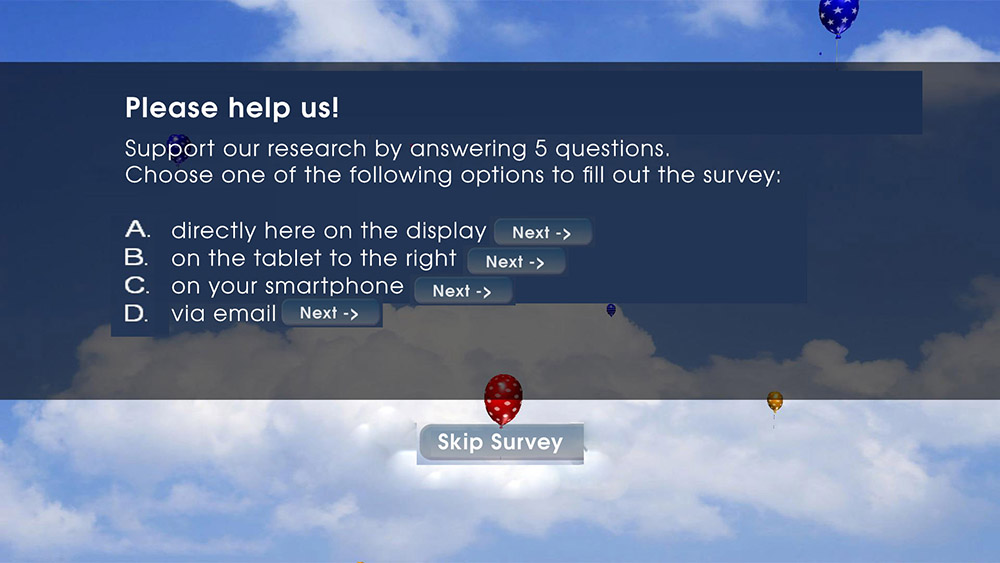
\includegraphics[width=\columnwidth]{img/screenshots/options-overview.jpg}
        \end{center}
     \caption{All four four options for completing a survey, the order being randomized on every instance.}
     \label{screenshot:options}
    \end{figure}


    1st option: tv screen

    \begin{figure}
        \begin{center}
            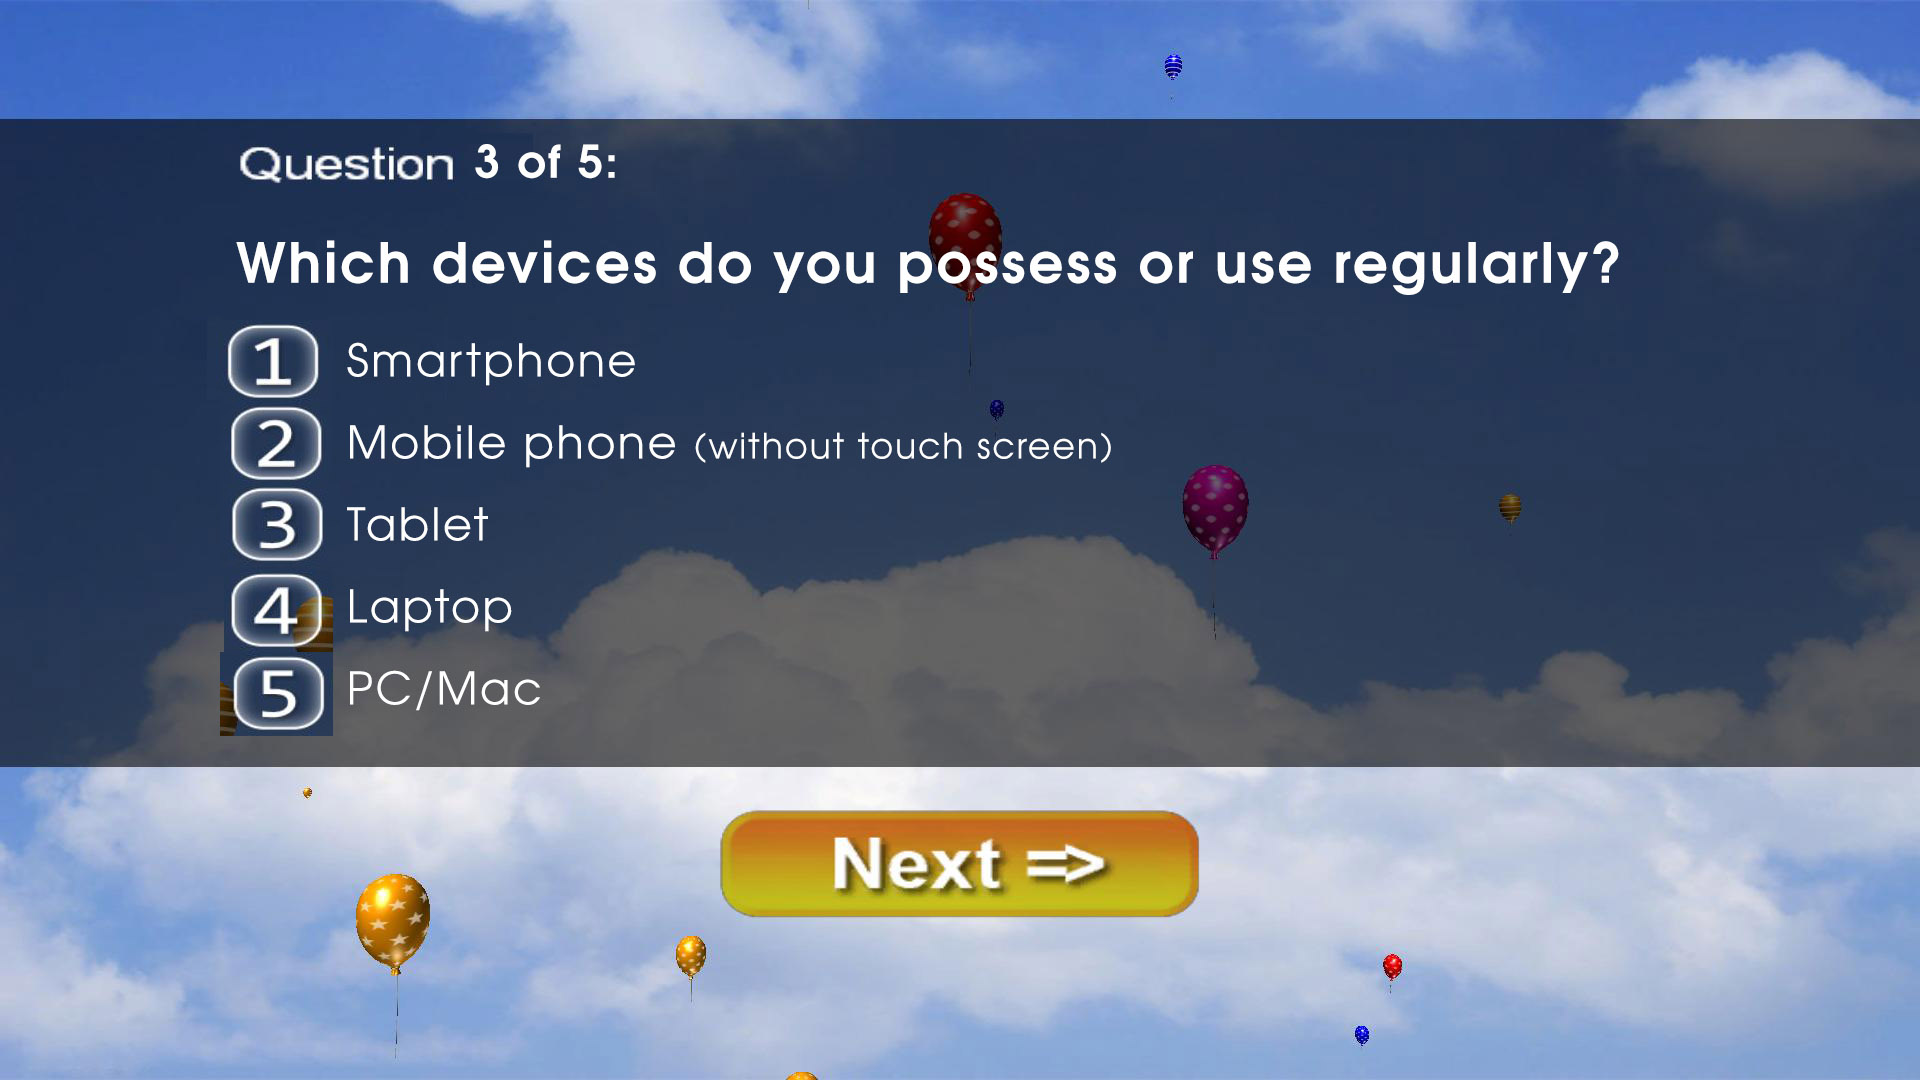
\includegraphics[width=\columnwidth]{img/screenshots/option-tv.jpg}
        \end{center}
     \caption{Option 1, directly answering on the TV screen. Here you see a sample question getting asked on the interactive display.}
     \label{screenshot:tv-option}
    \end{figure}


    2nd option: tablet

    \begin{figure}
        \begin{center}
            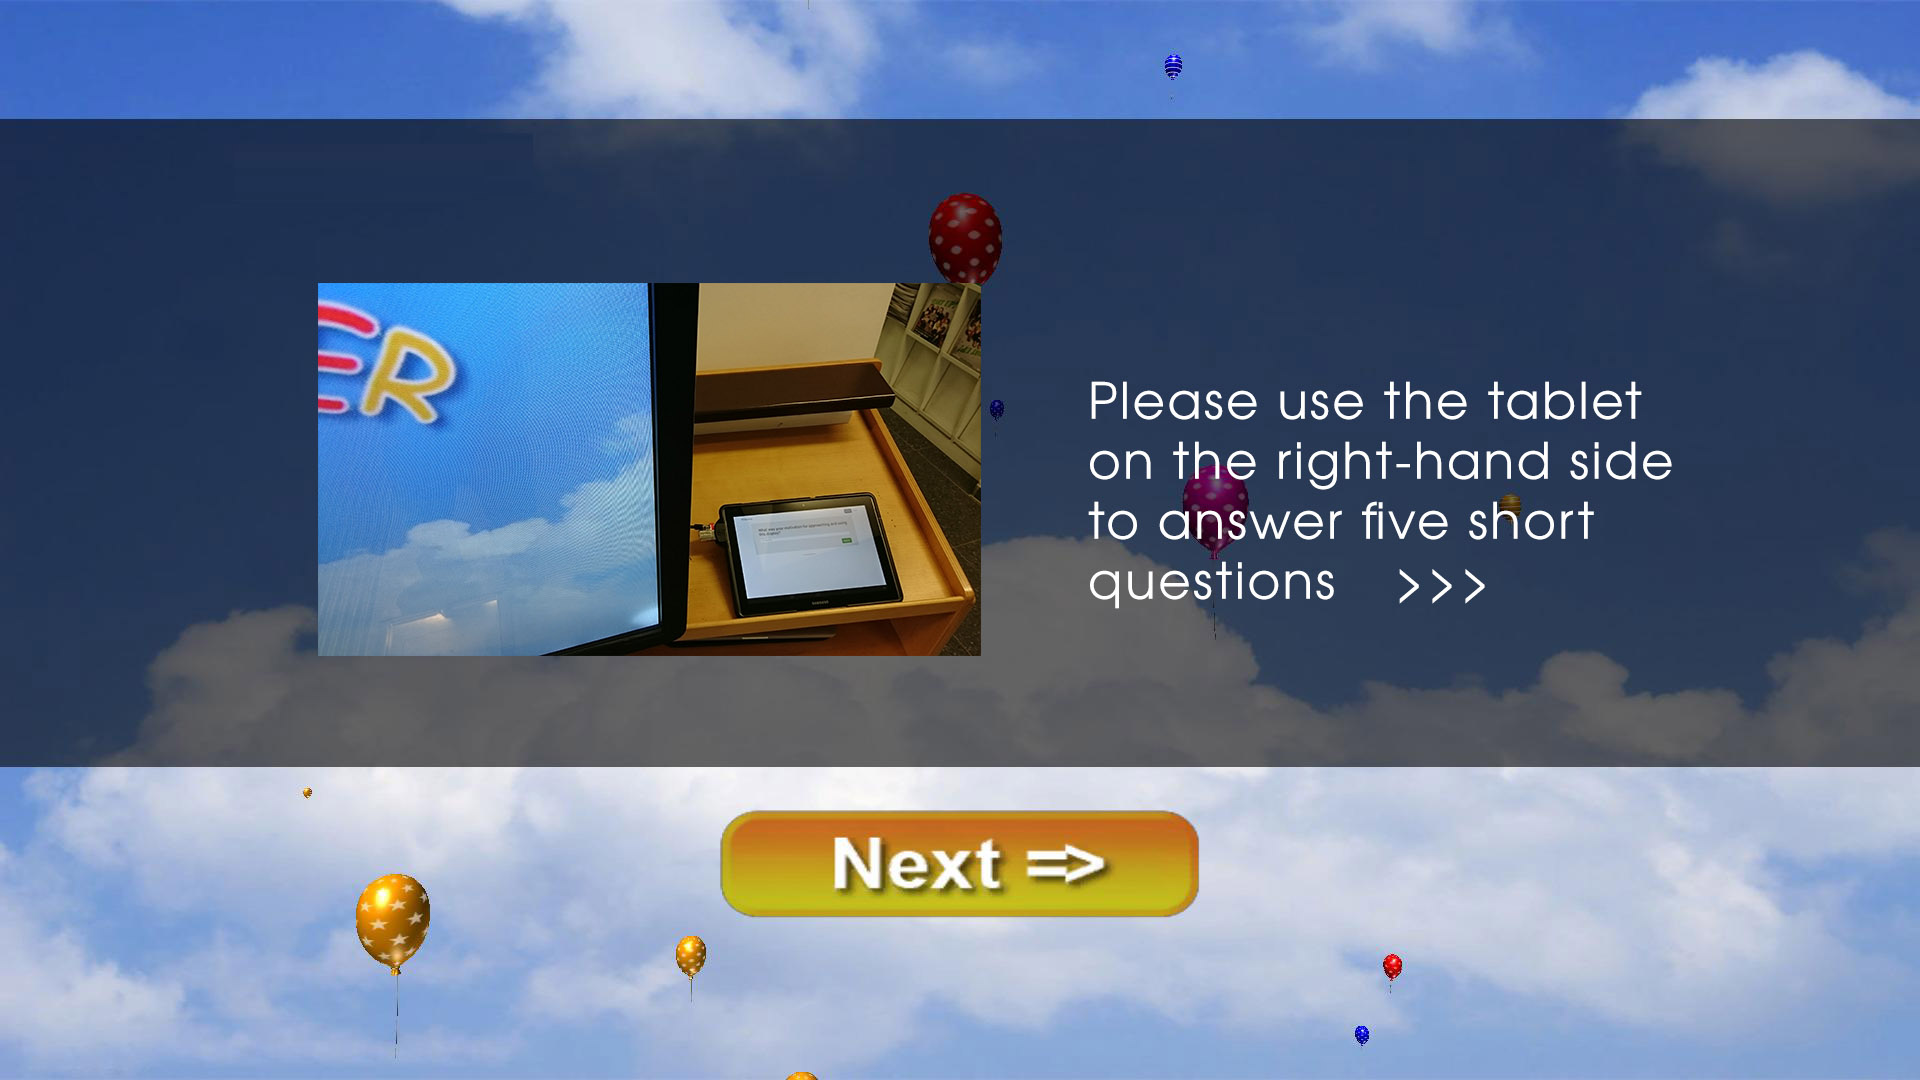
\includegraphics[width=\columnwidth]{img/screenshots/option-tablet.jpg}
        \end{center}
     \caption{Option 2, the screen the user sees when choosing to complete the survey on the tablet.}
     \label{screenshot:tablet-option}
    \end{figure}


    3rd option: smartphone

    \begin{figure}
        \begin{center}
            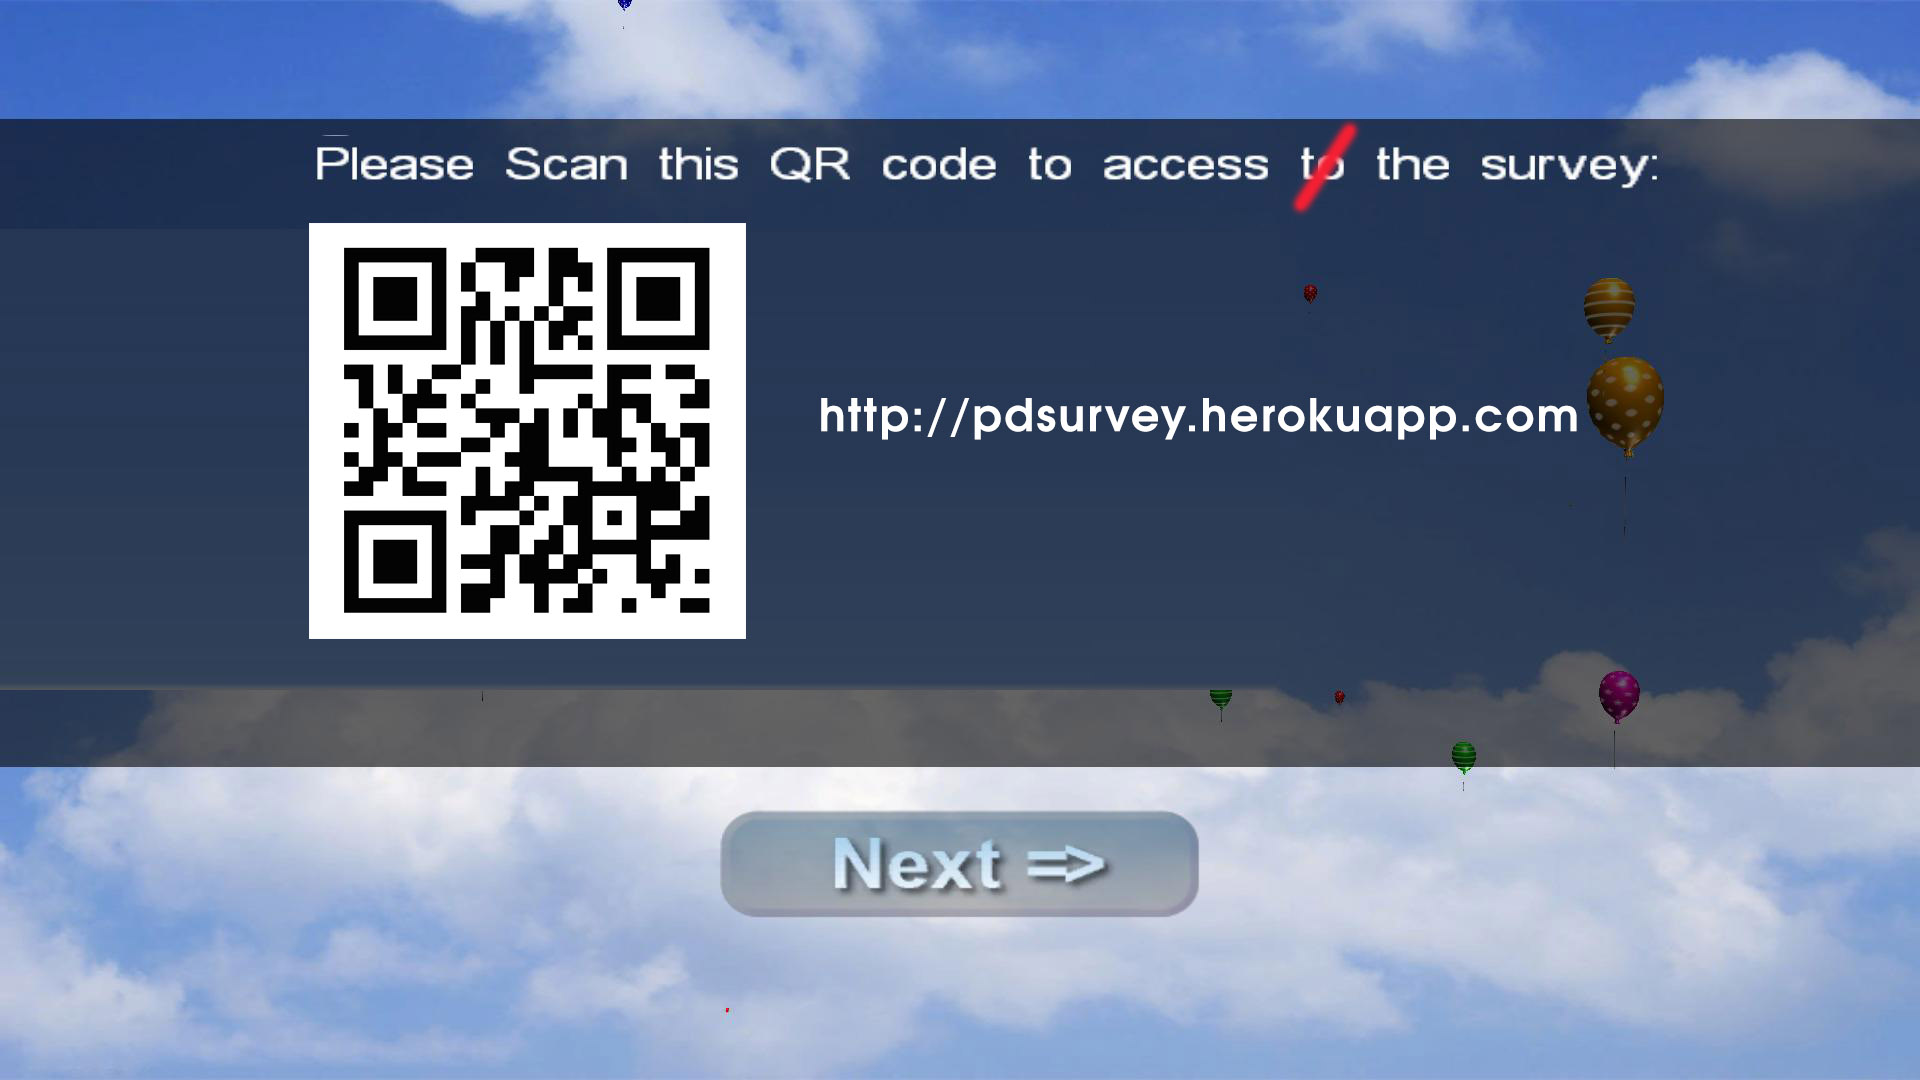
\includegraphics[width=\columnwidth]{img/screenshots/option-smartphone.jpg}
        \end{center}
     \caption{Option 3, participating with your own smartphone, either by scanning the QR code or by typing the URL in the mobile browser.}
     \label{screenshot:smartphone-option}
    \end{figure}


    4th option: email

    \begin{figure}
        \begin{center}
            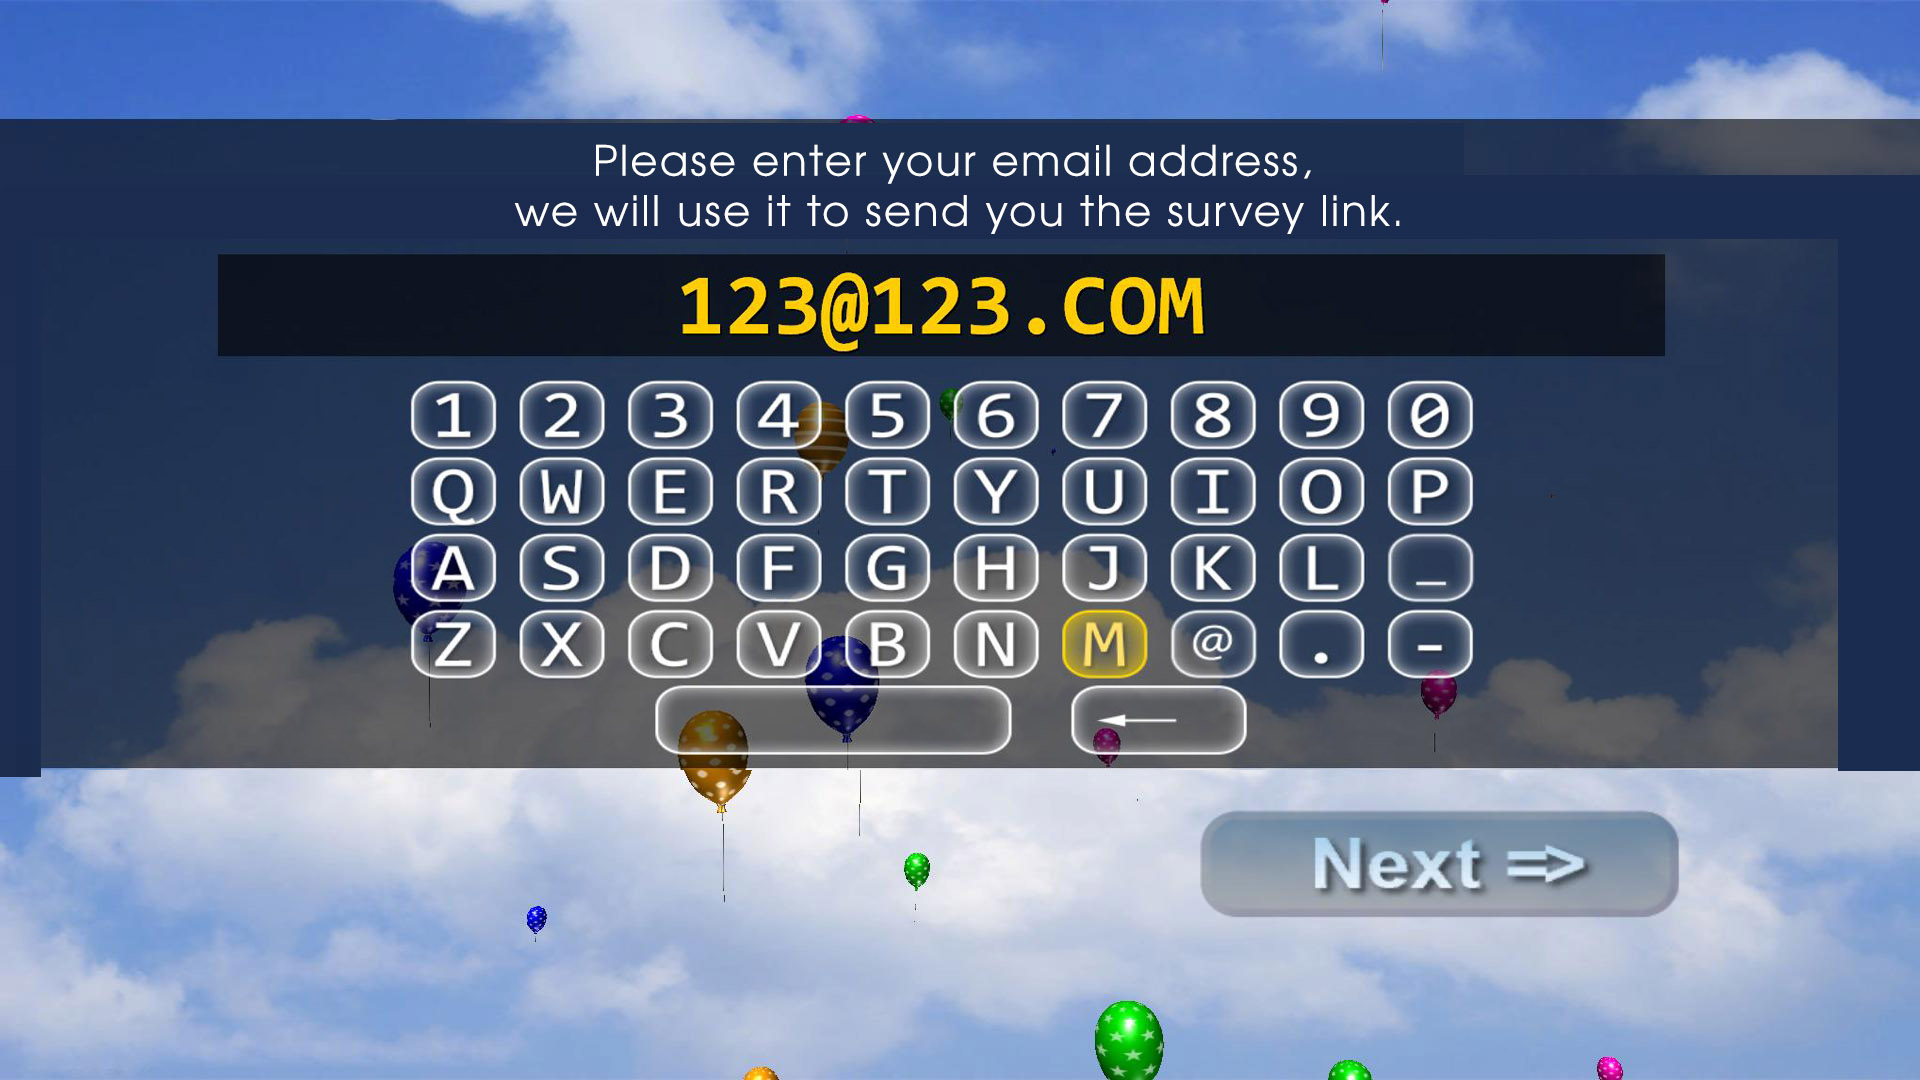
\includegraphics[width=\columnwidth]{img/screenshots/option-email.jpg}
        \end{center}
     \caption{Option 4, submitting ones email address and getting the survey link to participate in response.}
     \label{screenshot:email-option}
    \end{figure}

%________________________________________________________

\cleardoublepage
\part*{Bibliography}
\addcontentsline{toc}{part}{Bibliography}


%%  Literature / BibTex  %%

\bibliographystyle{plain}
\bibliography{literature}{} % import 'literature.bib'

\end{document}